\section{Normalized Radar Backscatter (NRB)}
\label{sec:nrb}

\subsection{Evaluation criteria}
\label{sec:nrb_criteria}
The evaluation of Normalised Radar Backscatter (\acs{nrb}) product is essential to ensure their suitability for downstream analysis. Key evaluation criteria include:

\begin{itemize}
    \item \textbf{Radiometric and Algorithm Consistency}: \acs{nrb} products should exhibit consistent radiometric values for similar targets, regardless of acquisition geometry (e.g., incidence angle), sensor mode, or processing software. This includes:
    \begin{itemize}
        \item Comparison across different software tools and algorithms;
        \item Stability of radiometric response over varying acquisition conditions.
    \end{itemize}
    \item \textbf{Removal of Terrain-Slope Effects}: correct removal of terrain-induced backscatter variations is a critical requirement. The \acs{nrb} should be independent of local topographic slopes, ensuring that radiometric differences reflect surface properties rather than geometry.  
    \item \textbf{Dependence on External Data}: \acs{nrb} accuracy is influenced by several external data sources, notably:
    \begin{itemize}
        \item Digital Elevation Model (\acs{dem}): the Area Normalization Factor (\acs{anf}) may vary depending on \acs{dem} resolution and accuracy.
        \item Orbital Information: variations in the orbital tube (different orbits over the same track) may also impact the \acs{anf} and hence the \acs{nrb} values.
    \end{itemize}
\end{itemize}

The geometric accuracy is primarily assessed on Coregistered Single Look Complex (\acs{cslc}) or Geocoded Single Look Complex (\acs{gslc}) products. The geocoding process used for \acs{nrb} products preserves spatial relationships and align features accurately with ground coordinates. The routines used to transform between radar and ground reference frames are the same as those applied during \acs{cslc}/\acs{gslc} generation. Therefore, \acs{nrb} geolocation accuracy is expected to match that of \acs{cslc}.

The impact of \acs{etad} information has been evaluated for \acs{cslc} product. The same advantages in terms of geolocation accuracy are inherited from the \acs{nrb} product.

The characteristics of the Impulse Response Function (\acs{irf}) are primarily evaluated using full resolution \acs{cslc} or \acs{gslc} products. These products allow for the precise identification of distortions in the \acs{irf}, which in turn reflect the expected accuracy of \acs{nrb} products.


\subsection{Radiometric and Algorithm Consistency}
\subsubsection{SW and algorithm comparison}
\label{sec:nrb_implementation_comparison}

One possible way to evaluate the radiometric and algorithmic consistency of a Normalized Radar Backscatter (\acs{nrb}) product is to compare the results in a challenging scenario such as a high-relief alpine area, using different algorithmic approaches and software implementations.

In this study, we assess two algorithmic approaches: point-based and area-based; each tested with two independent software implementations.

\begin{itemize}
  \item \textbf{Area-Based NRB Algorithm \cite{Shiroma2022}}: this algorithm aims to correct the backscatter by calculating the effective illuminated area for each ground pixel using a Digital Elevation Model (DEM). This approach typically involves projecting ground pixels to radar coordinates, calculating the corresponding area in radar geometry, and normalizing the backscatter by this area.
    \begin{itemize}
      \item OPERA–ISCE3 (C/C++) \url{https://github.com/opera-adt/RTC}
      \item Sentinel-1 Re-engineering (Python) by B-Open (S1-RP)
    \end{itemize}
  \item \textbf{Point-Based NRB Algorithm \cite{Small2011}}: this algorithm uses point like corrections. This typically involves identifying the radar coordinates for specific ground points and applying corrections based on the local incidence angle of multiple ground cells involved in the same radar cell.
    \begin{itemize}
      \item Original C code by David Small (C-Code)
      \item SARSEN (Python) \url{https://github.com/bopen/sarsen}
    \end{itemize}
\end{itemize}

The following metrics are used to quantify time performance and similarity of the results:

\begin{enumerate}
  \item \textit{Processing Time}
  \item \textit{NRB statistics}
\end{enumerate}

\paragraph{Processing Time}

The tests over an alpine area in Italy generated \acs{nrb} products from 27 Sentinel-1 bursts in both VV and VH polarizations, each processed at 10 m and 30 m resolution.

Each of the software tools and the corresponding algorithm implementations was run on an Intel Ultra 9 185H with 16 cores and 48GB of RAM.

The following table summarizes the measured processing times.

\begin{longtblr}[
	label=tab:processing_time_cmp,
	entry = none,
	caption = {SW \& Algorithm Comparison: Processing Time},
	]{
		width=\linewidth,
		colspec = {Q[l,24]Q[c,19]Q[c,19]Q[c,19]Q[c,19]},
		vline{2-5} = {-}{},
		%vline{5-5} = {-}{},
		hlines,
		hline{1-Z} = {-}{0.05em},
		rowhead=2,
	}
	\SetCell[r=2]{l} \textbf{\#processed bursts \& product resolution} & \SetCell[c=2]{c} \textbf{Area-Based Algorithm} & & \SetCell[c=2]{c} \textbf{Point-Based Algorithm}& & \\
	& \textbf{OPERA–ISCE3} & \textbf{B-Open \\ S1-RP} & \textbf{Small \\ C-Code} & \textbf{B-Open \\ SARSEN} \\
    27 Burst VV + VH 10 m & 1h 21m 27s & 45m 47s & 31m & 25m 45s \\
    27 Burst VV + VH 30 m & 26m & 15m 22s & 8m & 8m 52s 
\end{longtblr}

Note that SARSEN simplifies some interpolation steps (e.g., by using a nearest-neighbour algorithm), which speeds up the software execution but results in products with lower performance.

\paragraph{NRB statistics}
\label{sec:nrb_stats}

The difference between two \acs{nrb} products obtained from Sentinel-1 data in an Alpine region, one acquired in ascending geometry and the other in descending, was evaluated using three software tools: OPERA-ISCE3, B-Open S1-RP, and the original Small C-Code.

Comparing OPERA-ISCE3 with B-Open S1-RP validates that both independent implementations of the area-based algorithm \cite{Shiroma2022}, despite differing languages and architectures, yield very consistent results. Including the Small C-Code, which implements the point-based algorithm \cite{Small2011}, allows us to assess the impact of using a different radiometric correction model. Figure~\ref{fig:nrbs_comparison} shows the root mean square difference (RMSD) between ascending and descending observations for each tool.

\begin{figure}[h!]
  \centering
    \centering
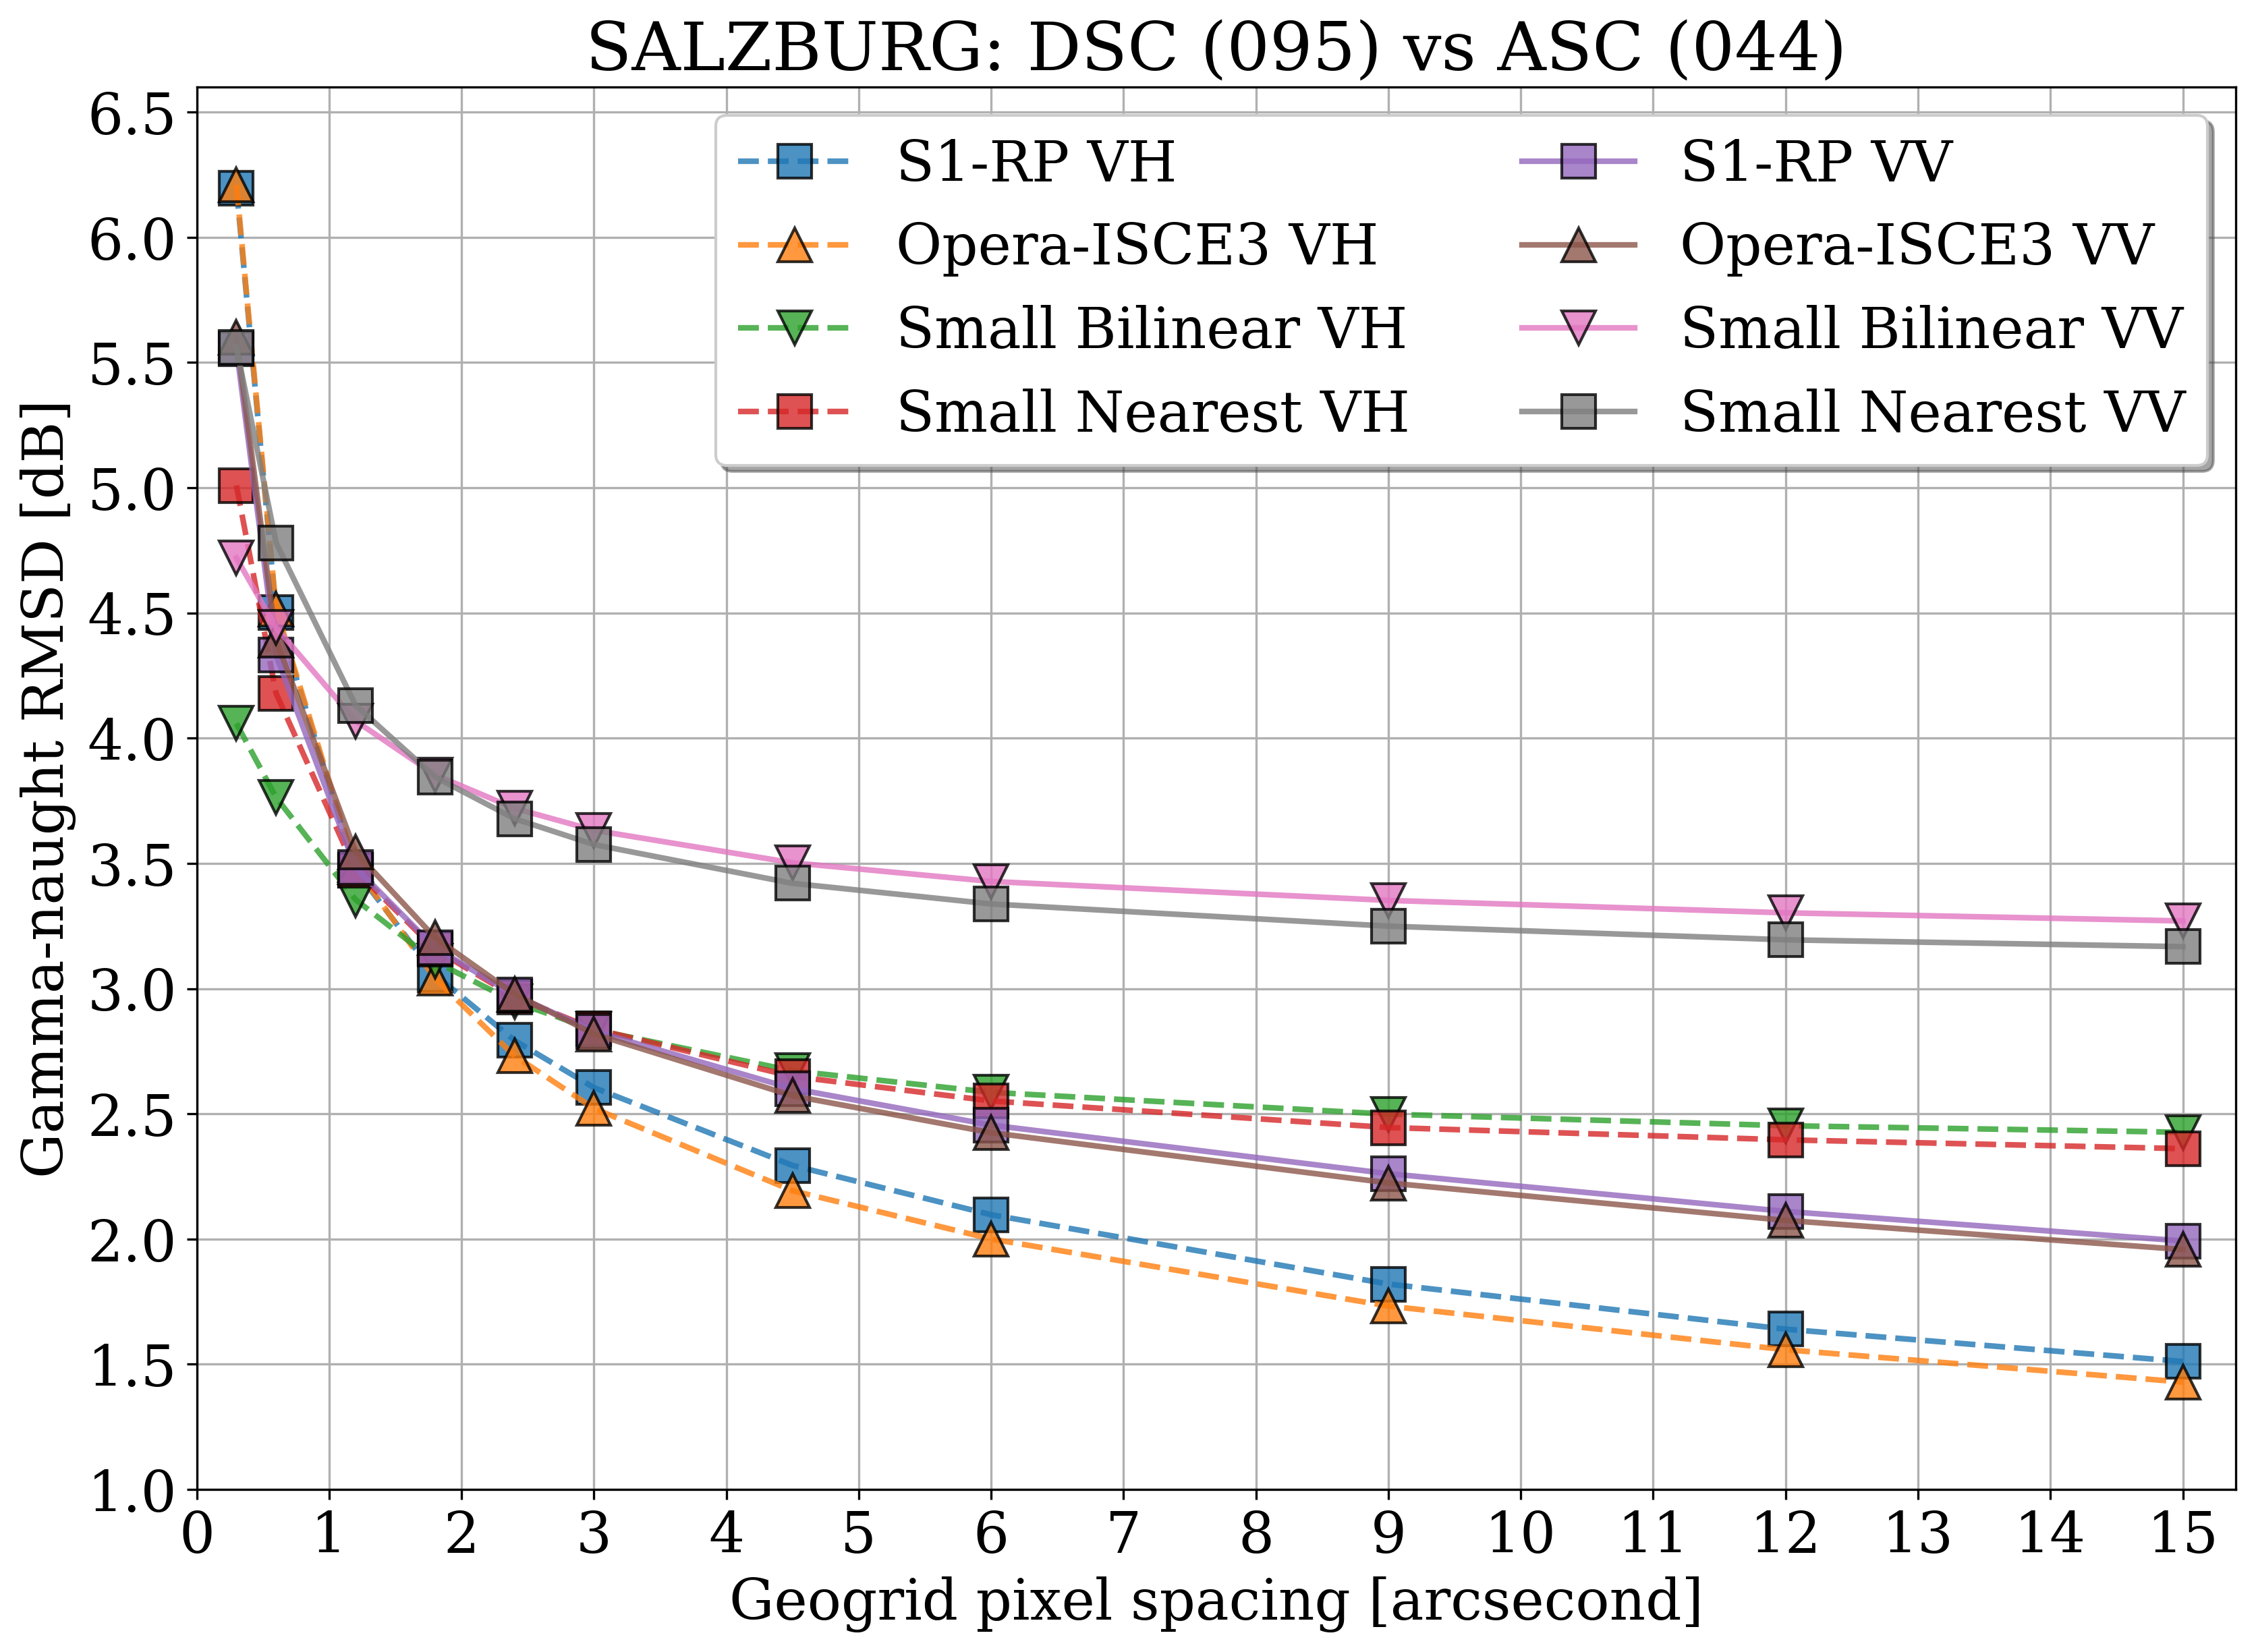
\includegraphics[width=0.9\textwidth]{Figures/nrb/new_salzburg.png}
    \caption{Root mean square difference between ascending and descending NRB products
over Salzburg, using COPDEM10m and multilooked resolutions from $0.3$ arcseconds up to $15$ arcseconds.}
    \label{fig:nrbs_comparison}
  \end{figure}

Figure~\ref{fig:nlooks_comparison} shows the histogram of the number of looks on the same area using \acs{s1rp}, OPERA-ISCE3 and the Small C-Code.

\begin{figure}[h!]
  \centering
    \centering
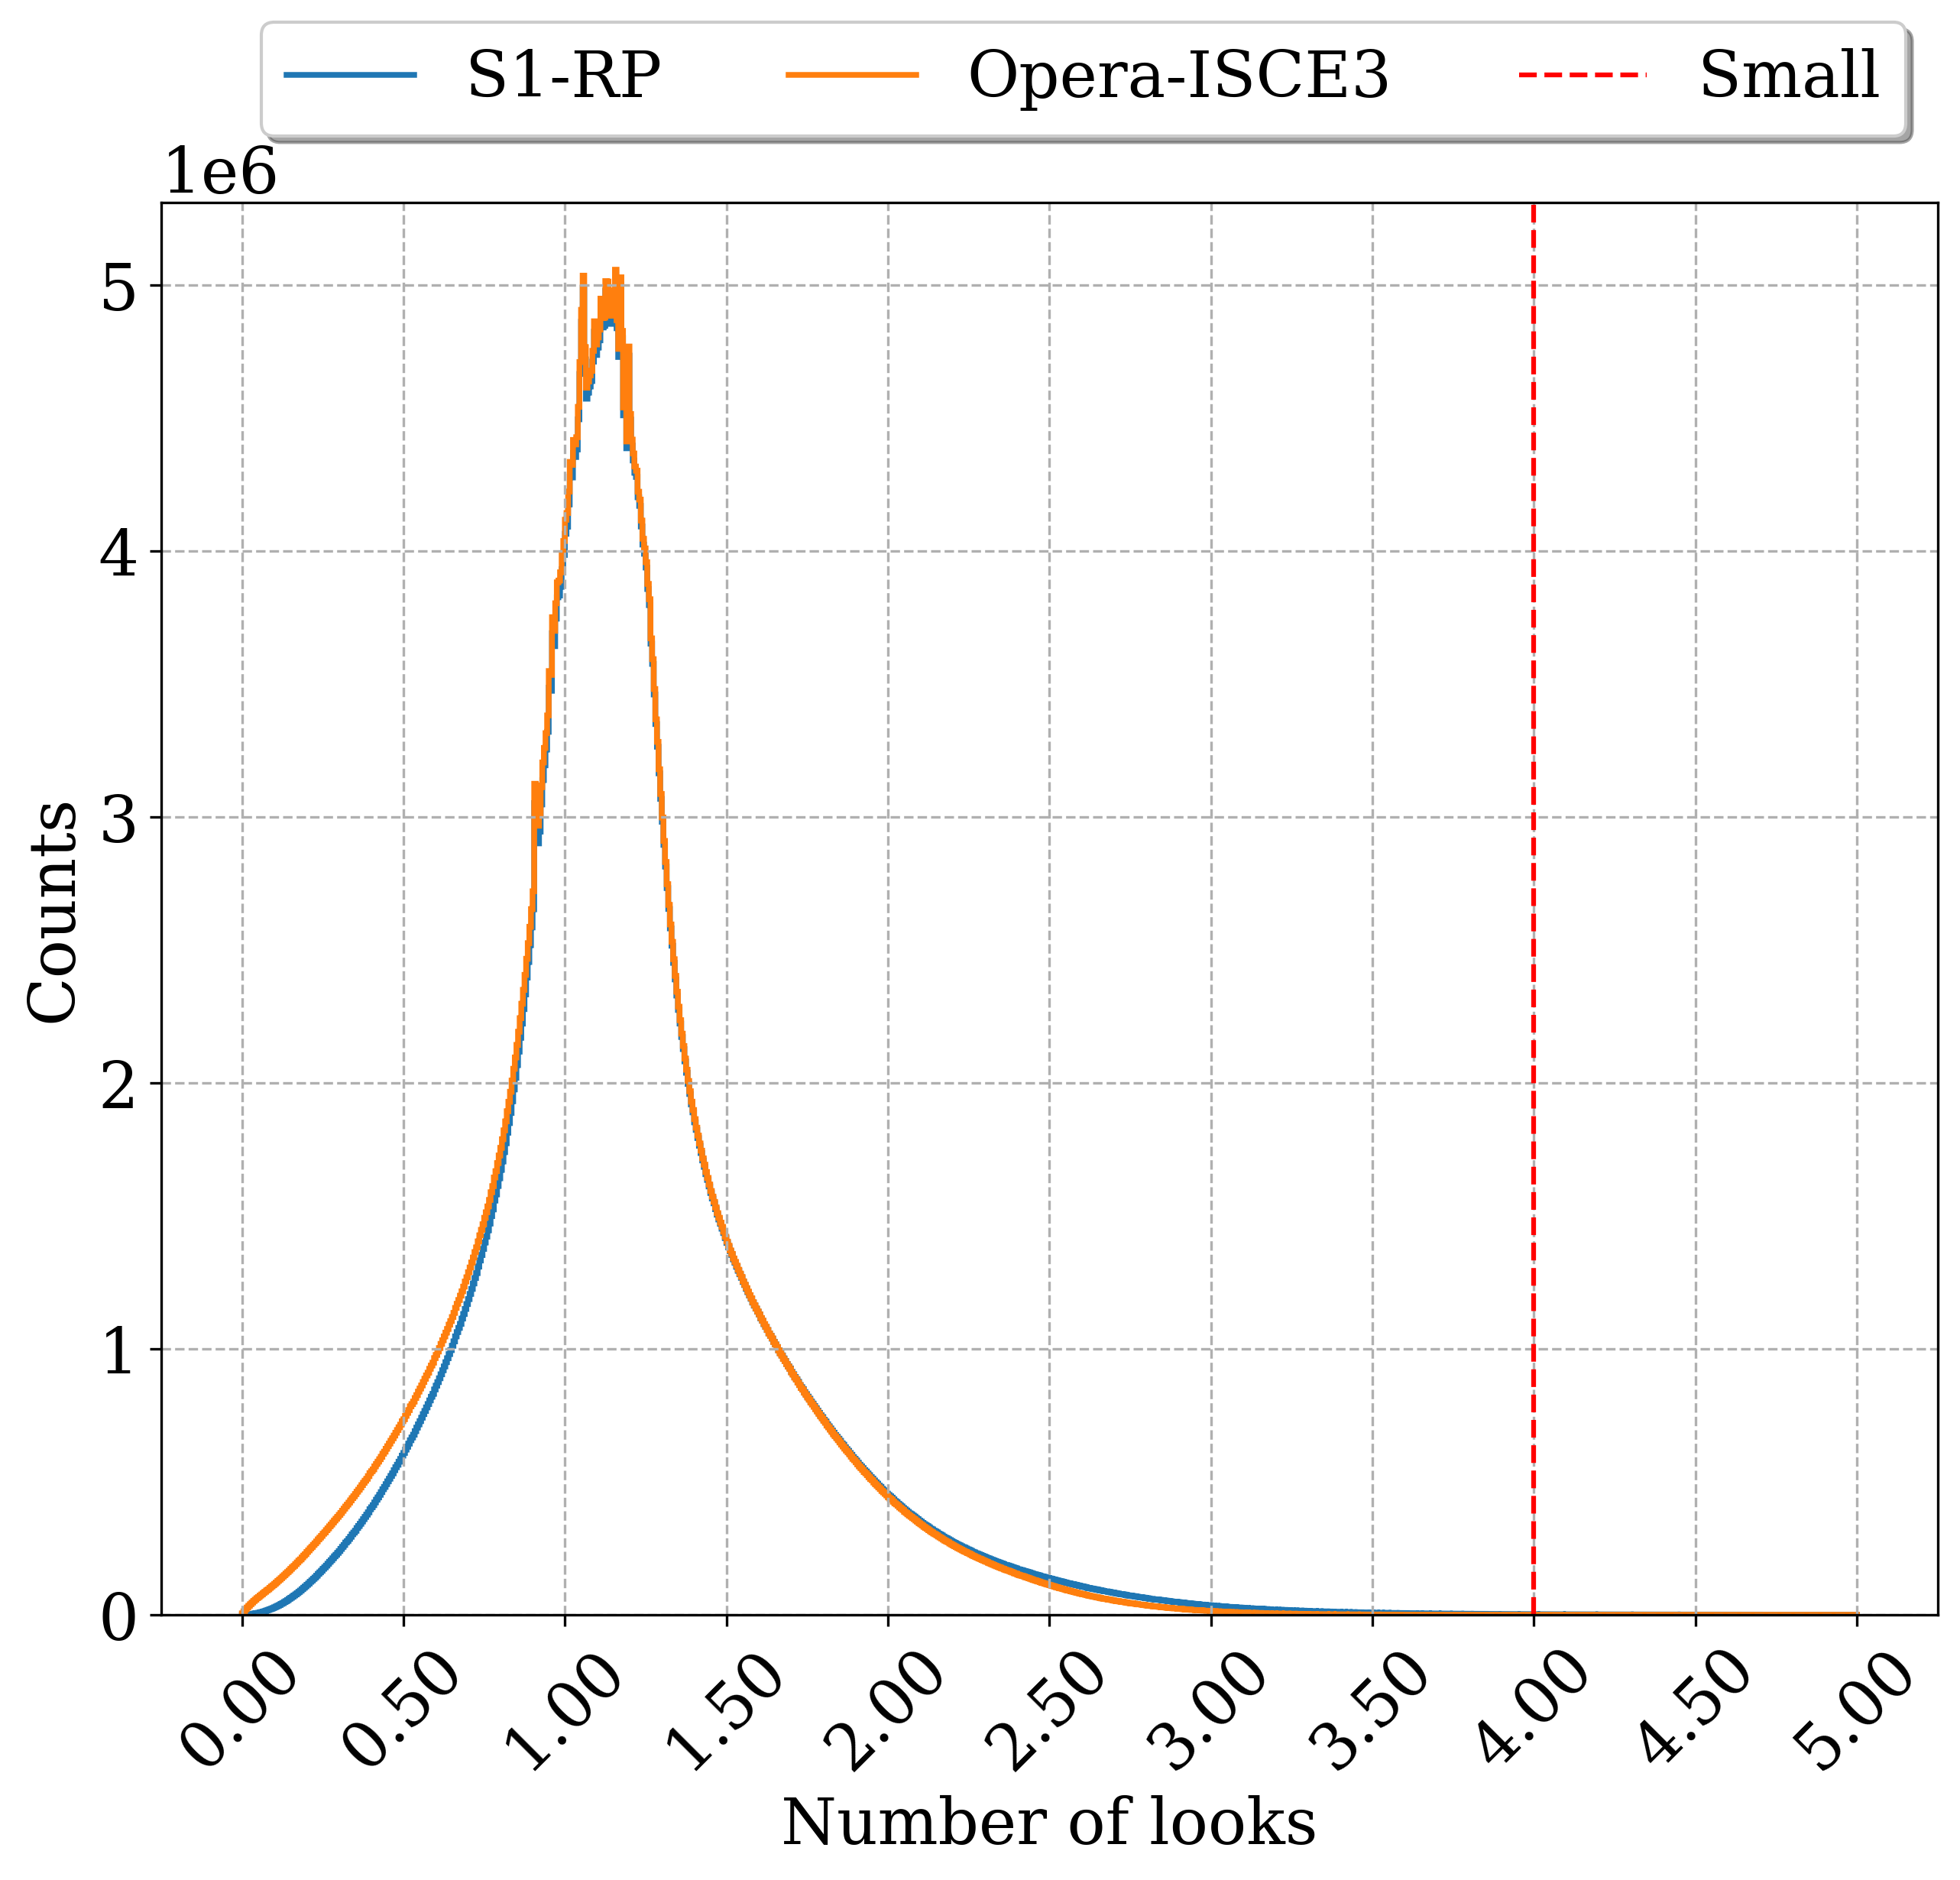
\includegraphics[width=0.7\textwidth]{Figures/nrb/nlooks_salzburg.png}
    \caption{Number of looks comparison on the same area between \acs{s1rp}, Opera-ISCE3 and Small C-Code.}
    \label{fig:nlooks_comparison}
  \end{figure}

As shown in Figure~\ref{fig:nlooks_comparison}, OPERA-ISCE3 and B-Open \acs{s1rp} produce perfectly aligned NRB products, with coincident RMSD values across all different output product spacing. In these area-based implementations, the effective multilook factor is dictated by the ground resolution and the radar to ground mapping geometry. In this example, at $0.3$ arcseconds ground sampling, the look count is approximately $1.12$ over flat terrain and increases with slope (which lowers speckle). Thus, at native resolution, speckle dominates the differences; as the effective number of looks grows (either by coarser sampling or explicit multilooking) the RMSD falls, and no systematic bias remains.

By contrast, the point-based C-Code inherently averages over a larger number of looks even at $0.3$ arcseconds resolution, yielding lower RMSD than the area-based tools (specifically, a constant multilook along both directions is performed, so that the aspect ratio is "squarish": in this example, a constant multilook of 4 along slant range, and a multilook of 1 along azimuth, have been performed). Furthermore, the bilinear interpolation step (recommended option) further increases the number of looks, and this is evident by comparing this approach with the Nearest Neighbor's one, as shown in Figure~\ref{fig:nrbs_comparison}.

However, when the output is coarsened by spatial averaging, the point-based algorithm still exhibits a residual bias of about 1 dB relative to the area-based algorithm. This remaining offset could reflects the different compensation model employed by the point-based approach.

\subsubsection{Stability of radiometric response over varying acquisition conditions}
\label{sec:nrb_stability_diff_geom}
The generation of \acs{nrb} products involves two main steps:

\begin{itemize}
    \item \textbf{\acs{anf} correction (gamma flattening)}: this step removes the dependency of the radar cross-section on the local terrain slope by applying a multiplicative compensation factor derived from a digital elevation model (DEM). It counteracts the radiometric distortions caused by foreshortening and shadowing.  
    \item \textbf{Geocoding}: this transforms data from radar geometry (slant range and azimuth) into ground coordinates (e.g.\ latitude, longitude) using the same projection matrix computed during the slope compensation stage.  
\end{itemize}

Figure~\ref{fig:Salzburg_044_VV_nocorr} shows a geocoded mosaicked NRB image over Salzburg without applying the \acs{anf} correction. Although the data are correctly projected, pixels located in foreshortened or layover zones appear artificially bright, while those in shadowed areas are unnaturally dark. After applying gamma flattening, as seen in Figure~\ref{fig:Salzburg_044_VV_corr}, these slope-induced radiometric artifacts are effectively removed, yielding a more uniform backscatter response across varying topography.

\begin{figure}[htbp]
  \centering
  \begin{subfigure}[b]{0.48\textwidth}
    \centering
    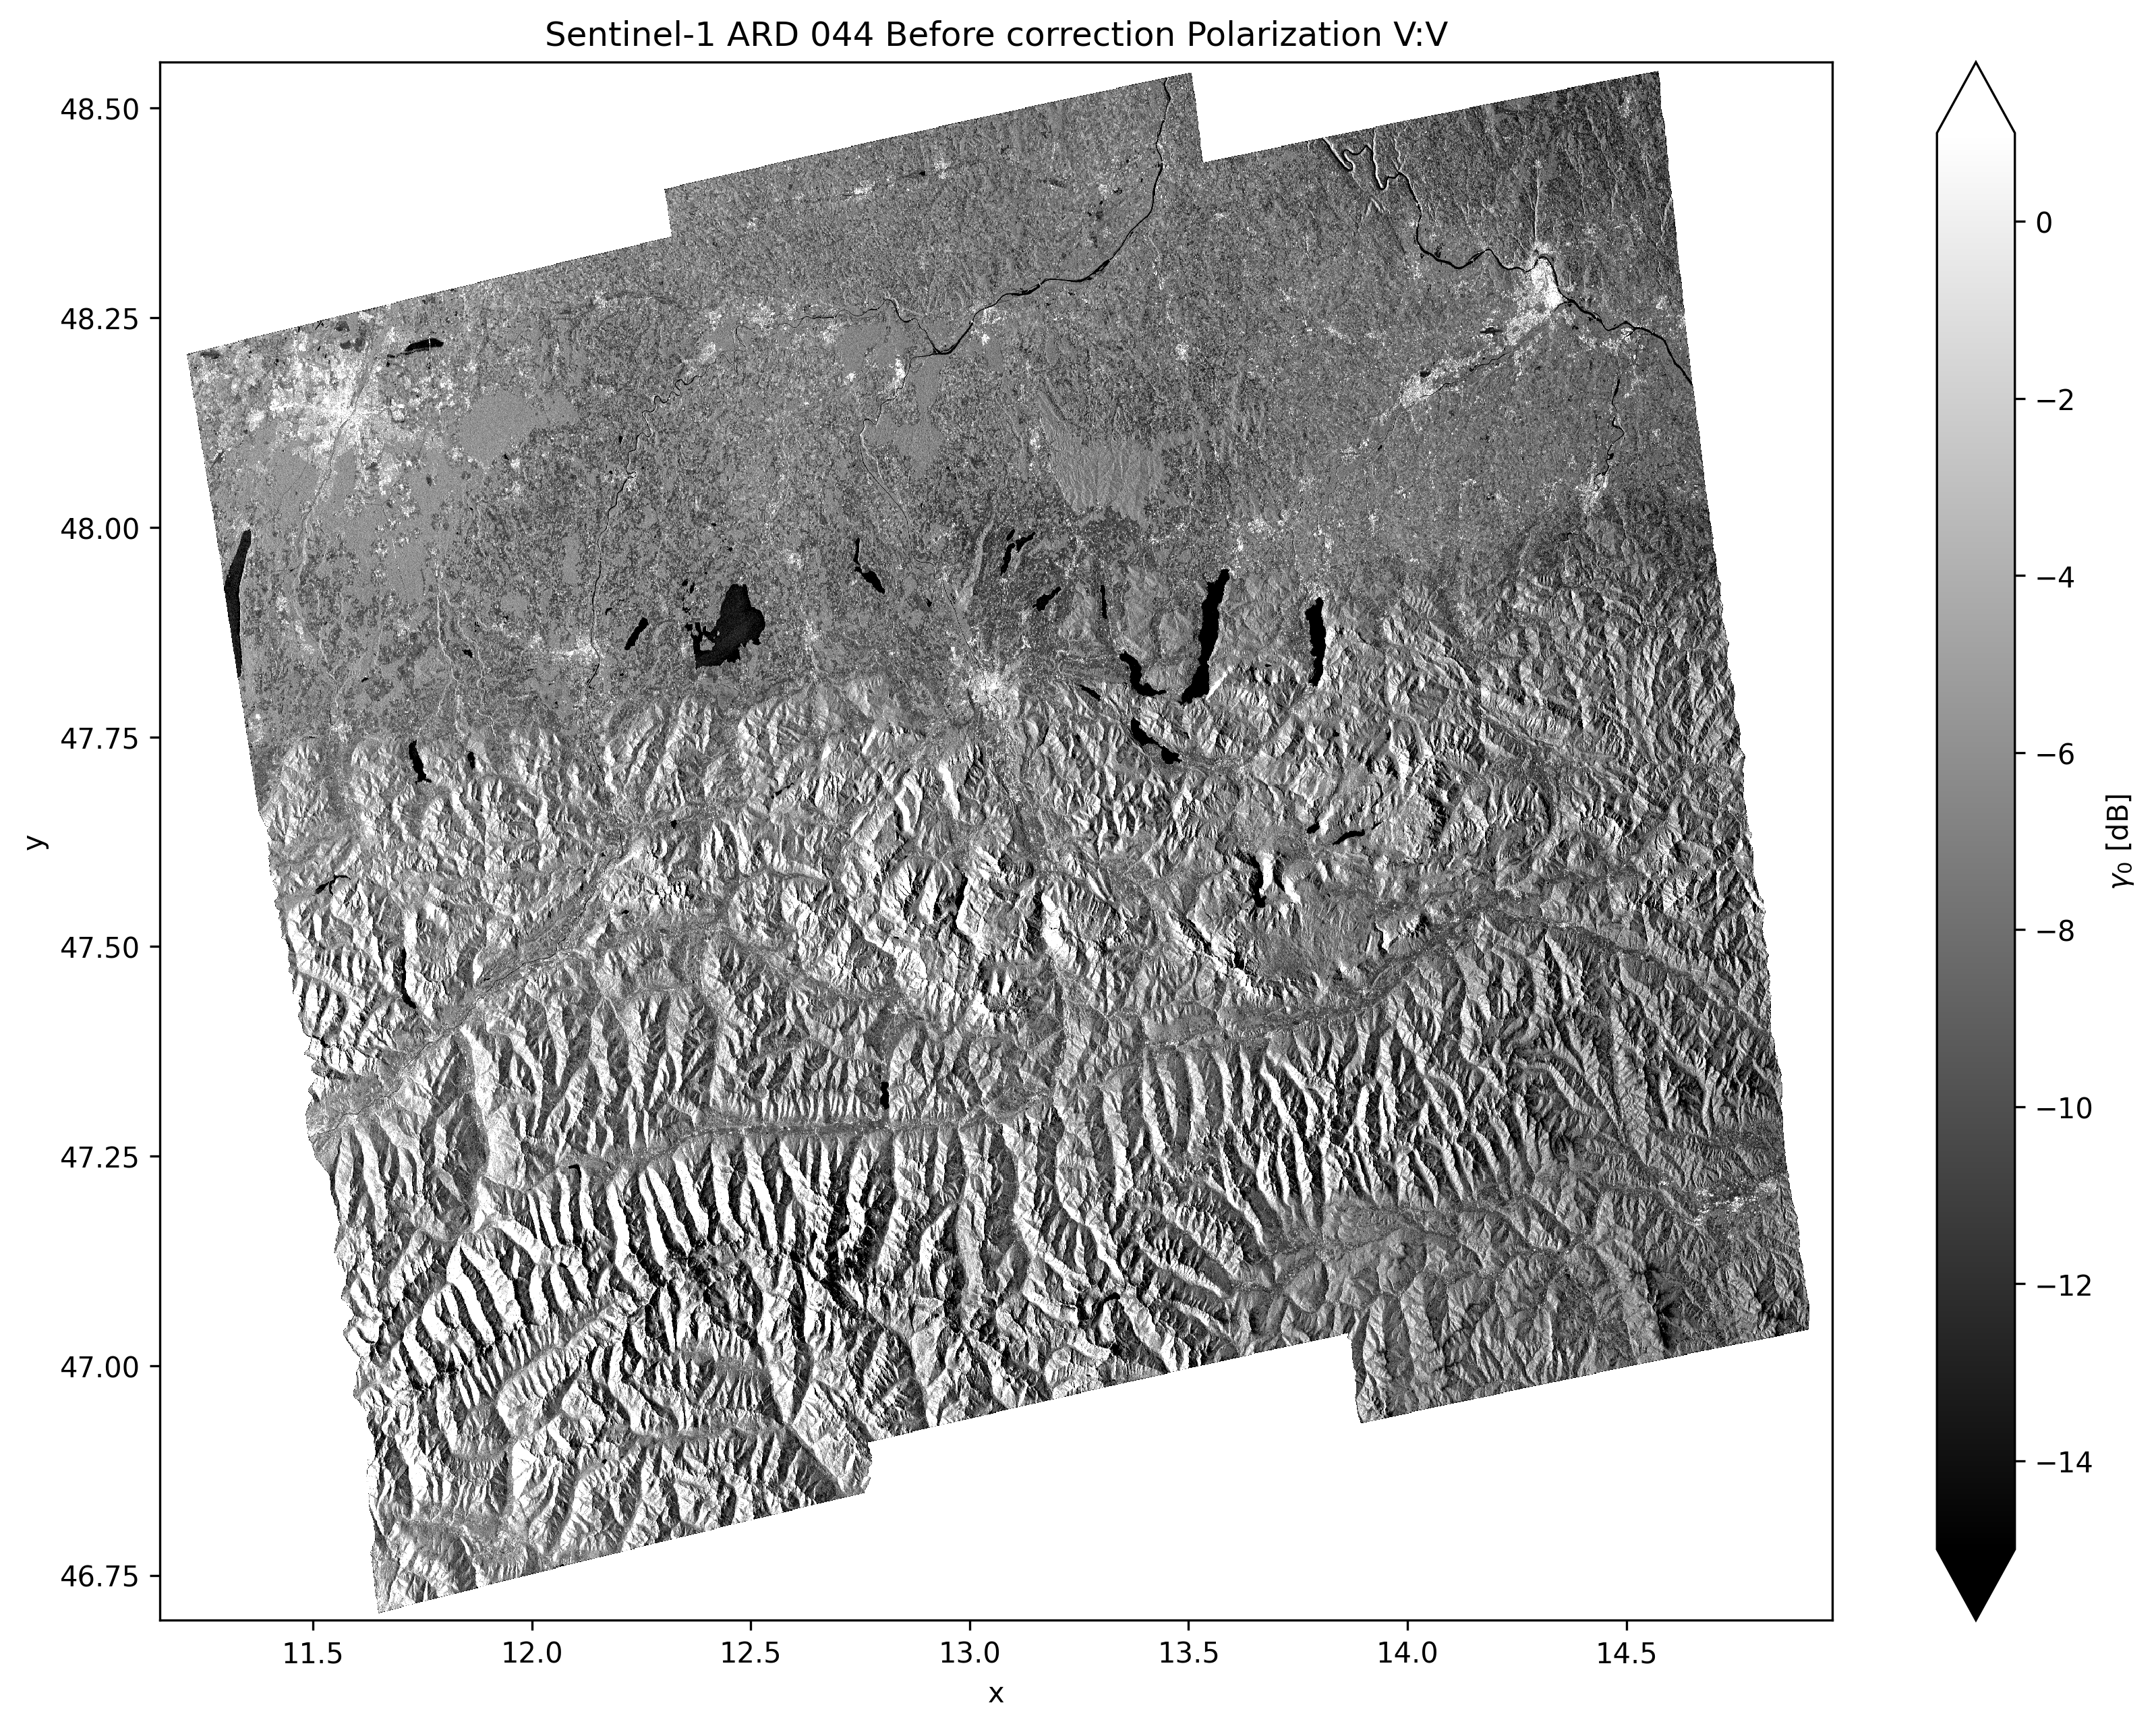
\includegraphics[width=\textwidth]{Figures/nrb/Salzburg_044_VV_nocorr.png}
    \caption{Without \acs{anf} correction}
    \label{fig:Salzburg_044_VV_nocorr}
  \end{subfigure}
  \hfill
  \begin{subfigure}[b]{0.48\textwidth}
    \centering
    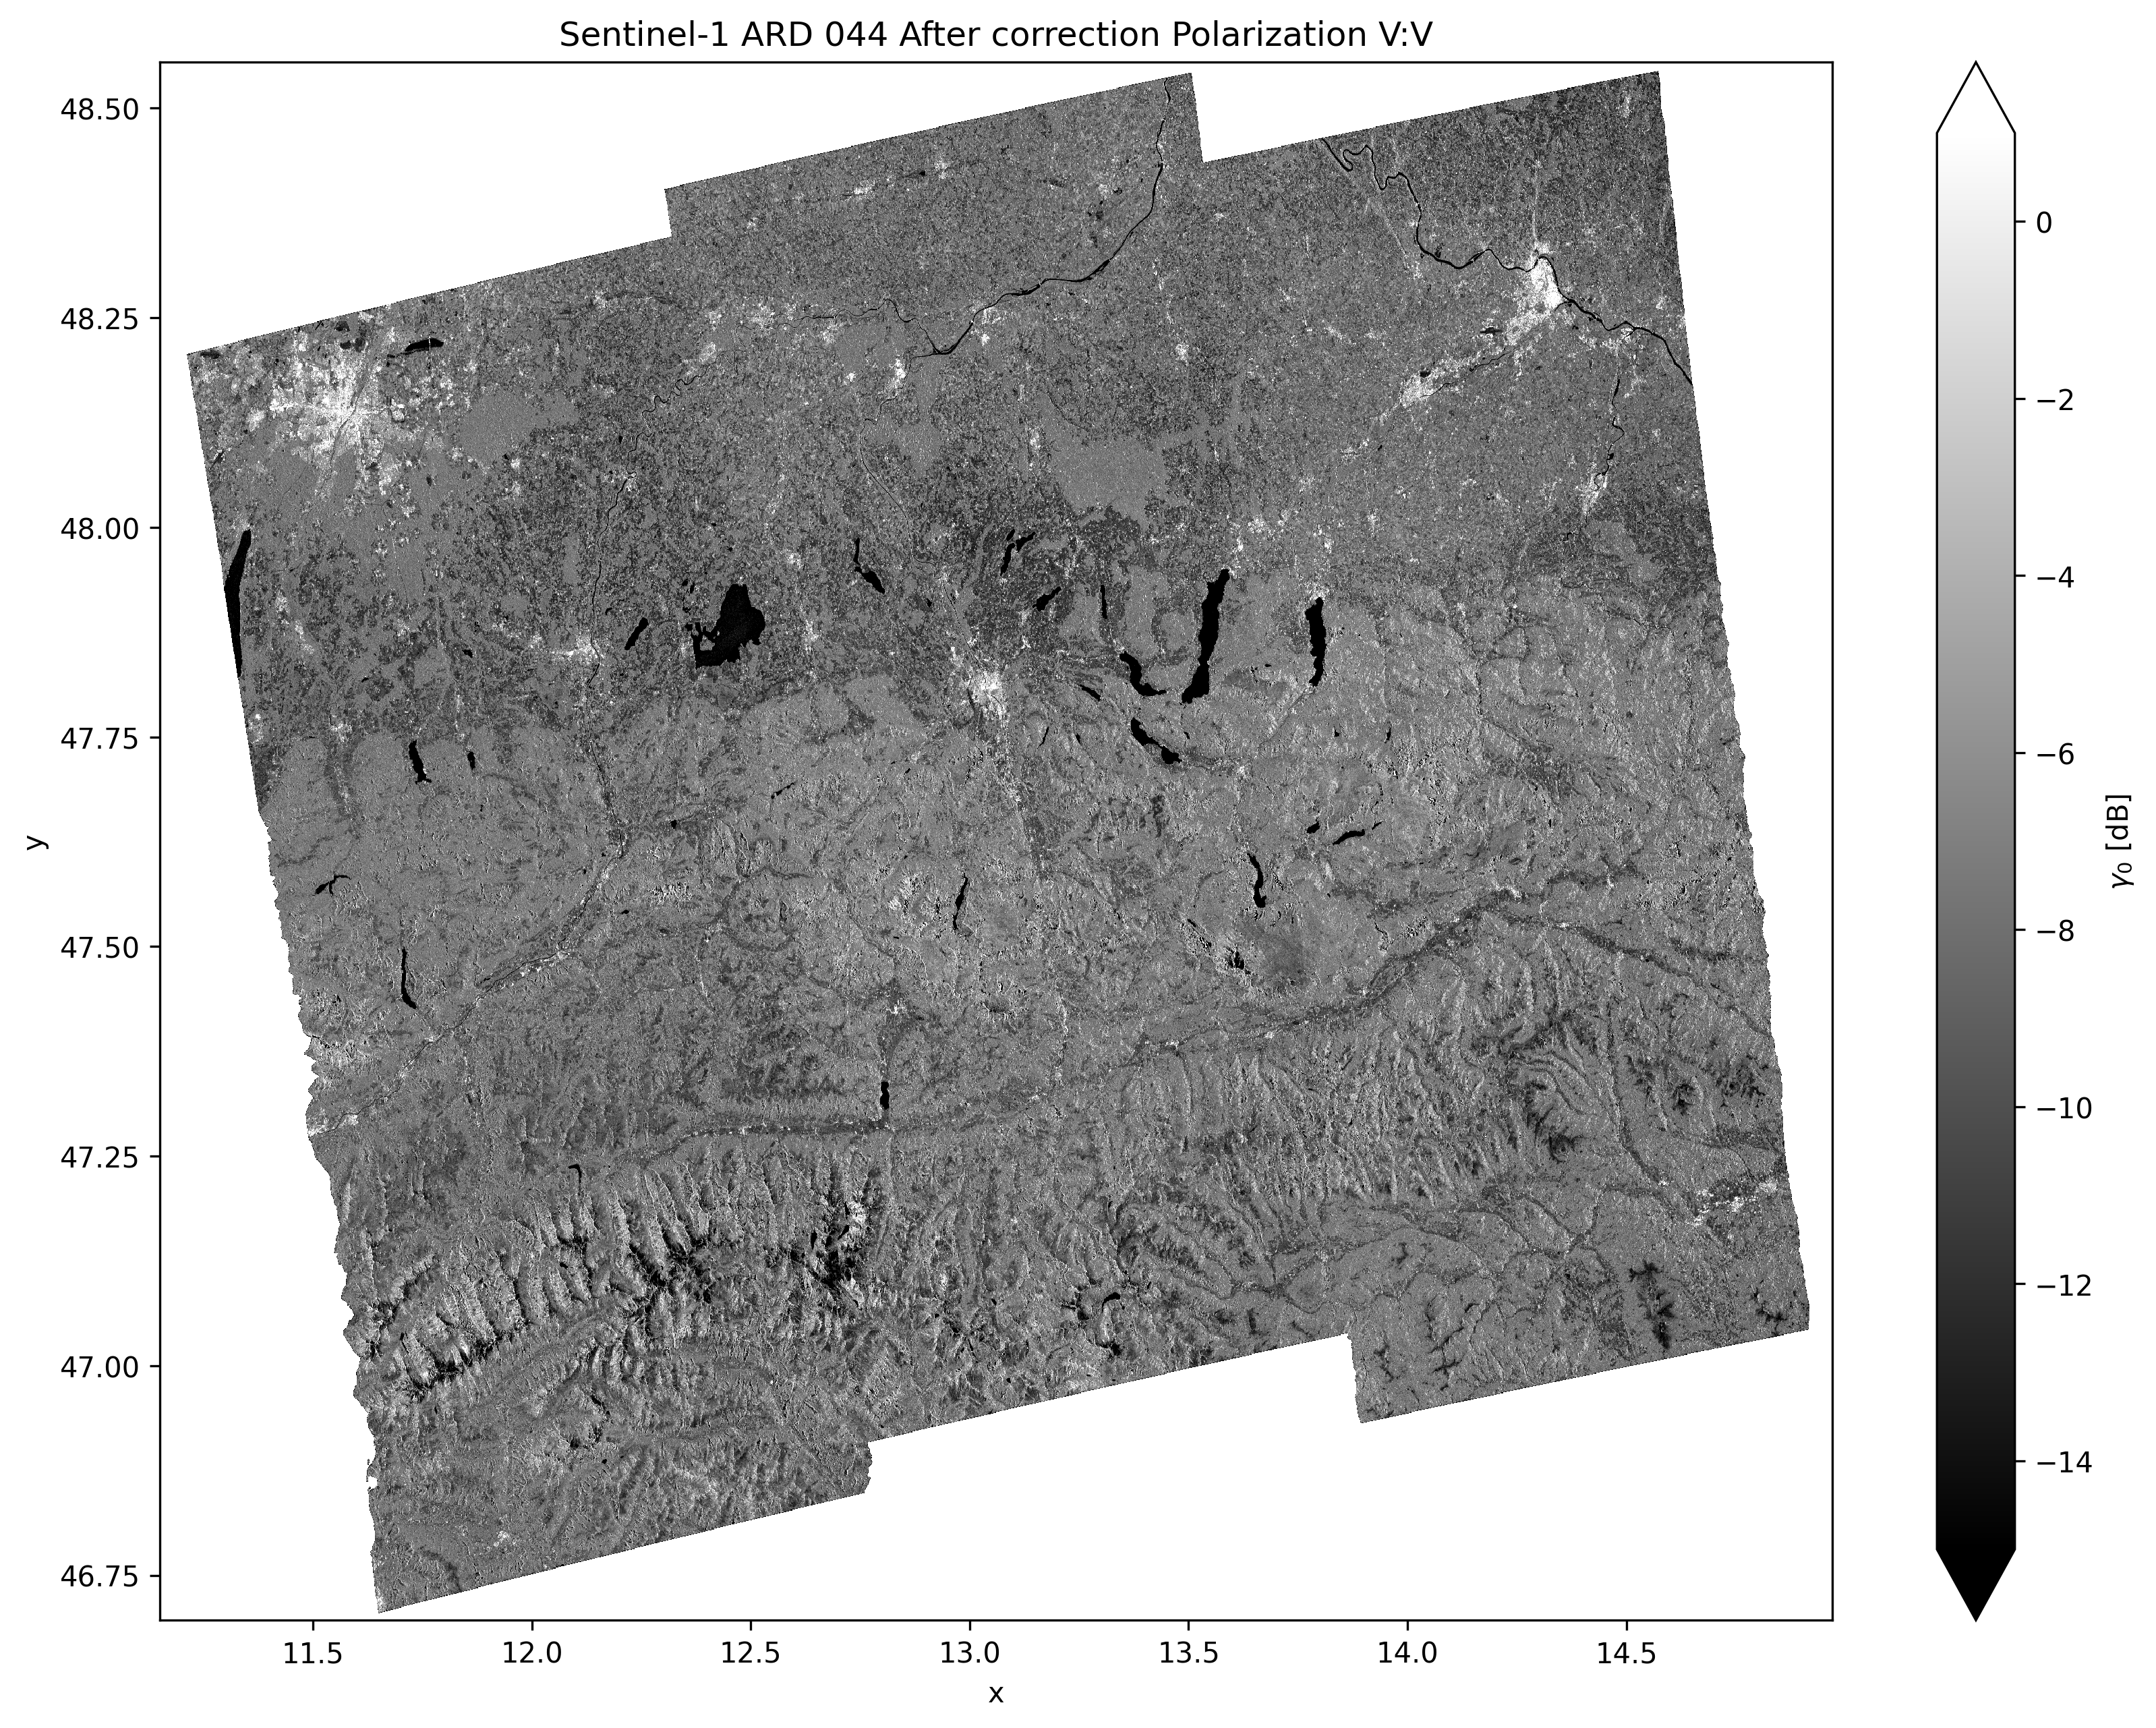
\includegraphics[width=\textwidth]{Figures/nrb/Salzburg_044_VV_corr.png}
    \caption{With \acs{anf} correction}
    \label{fig:Salzburg_044_VV_corr}
  \end{subfigure}
  \caption{Mosaicked NRB images of Salzburg before (left) and after (right) terrain slope flattening.}
  \label{fig:due_subfigure}
\end{figure}
This visual inspection provides qualitative insight only. To quantify the effectiveness of slope removal, we designed two tests:

\begin{itemize}
    \item \textit{Correlation index between NRB and terrain slope}  
    \item \textit{Slope compensation consistency across acquisition geometries}
\end{itemize}

\paragraph{Correlation index between NRB and terrain slope}

We processed a Sentinel-1 dataset over a steep alpine region twice: once including the slope compensation stage and once omitting it. For each version, we derived the local slope angle from a high-resolution DEM and constructed two-dimensional histograms of NRB values versus slope angle. This approach highlights any residual coupling between backscatter intensity and topography.

Figure~\ref{fig:hist_2d_no_corr} presents the histogram without compensation, where a clear diagonal band indicates that steeper terrain systematically biases the backscatter—higher incidence angles yield consistently different NRB values. Figure~\ref{fig:hist_2d_corr} shows the histogram after flattening: the diagonal structure nearly vanishes and NRB values distribute uniformly across all slopes, demonstrating effective removal of topographic dependency.

\begin{figure}[htbp]
  \centering
  \begin{subfigure}[b]{0.48\textwidth}
    \centering
    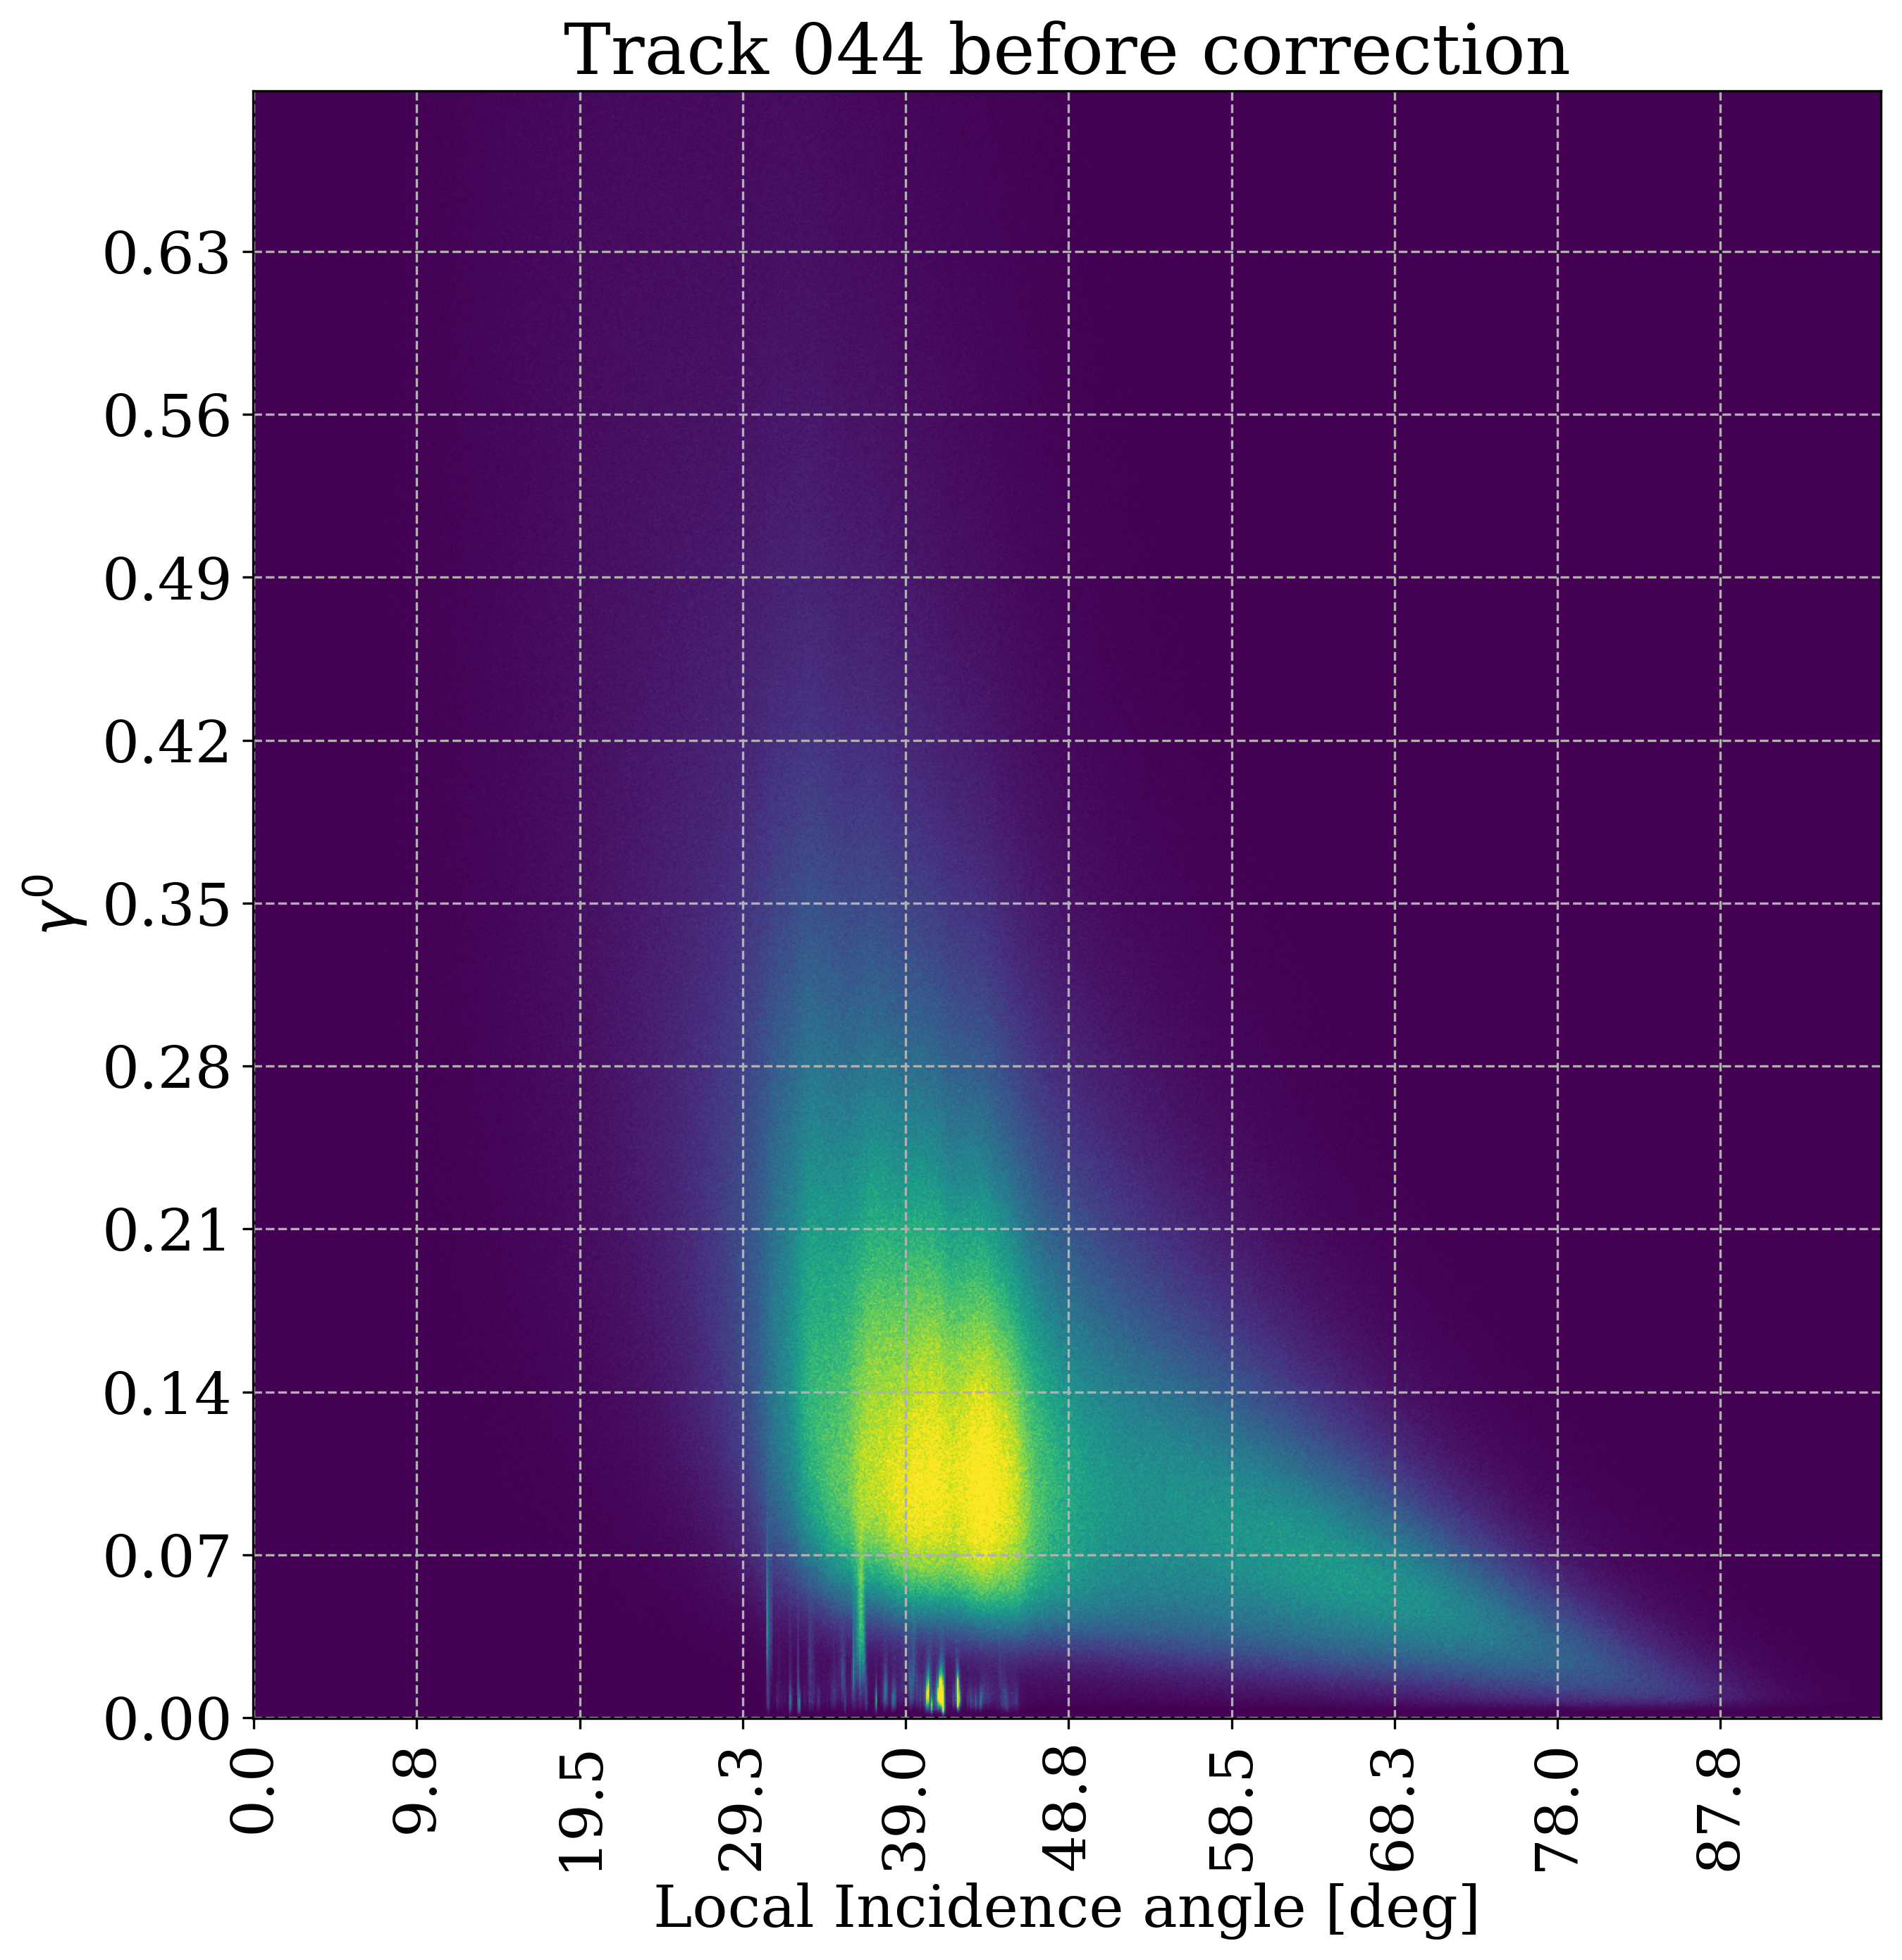
\includegraphics[width=\textwidth]{Figures/nrb/hist_2d_no_corr.png}
    \caption{}
    \label{fig:hist_2d_no_corr}
  \end{subfigure}
  \hfill
  \begin{subfigure}[b]{0.48\textwidth}
    \centering
    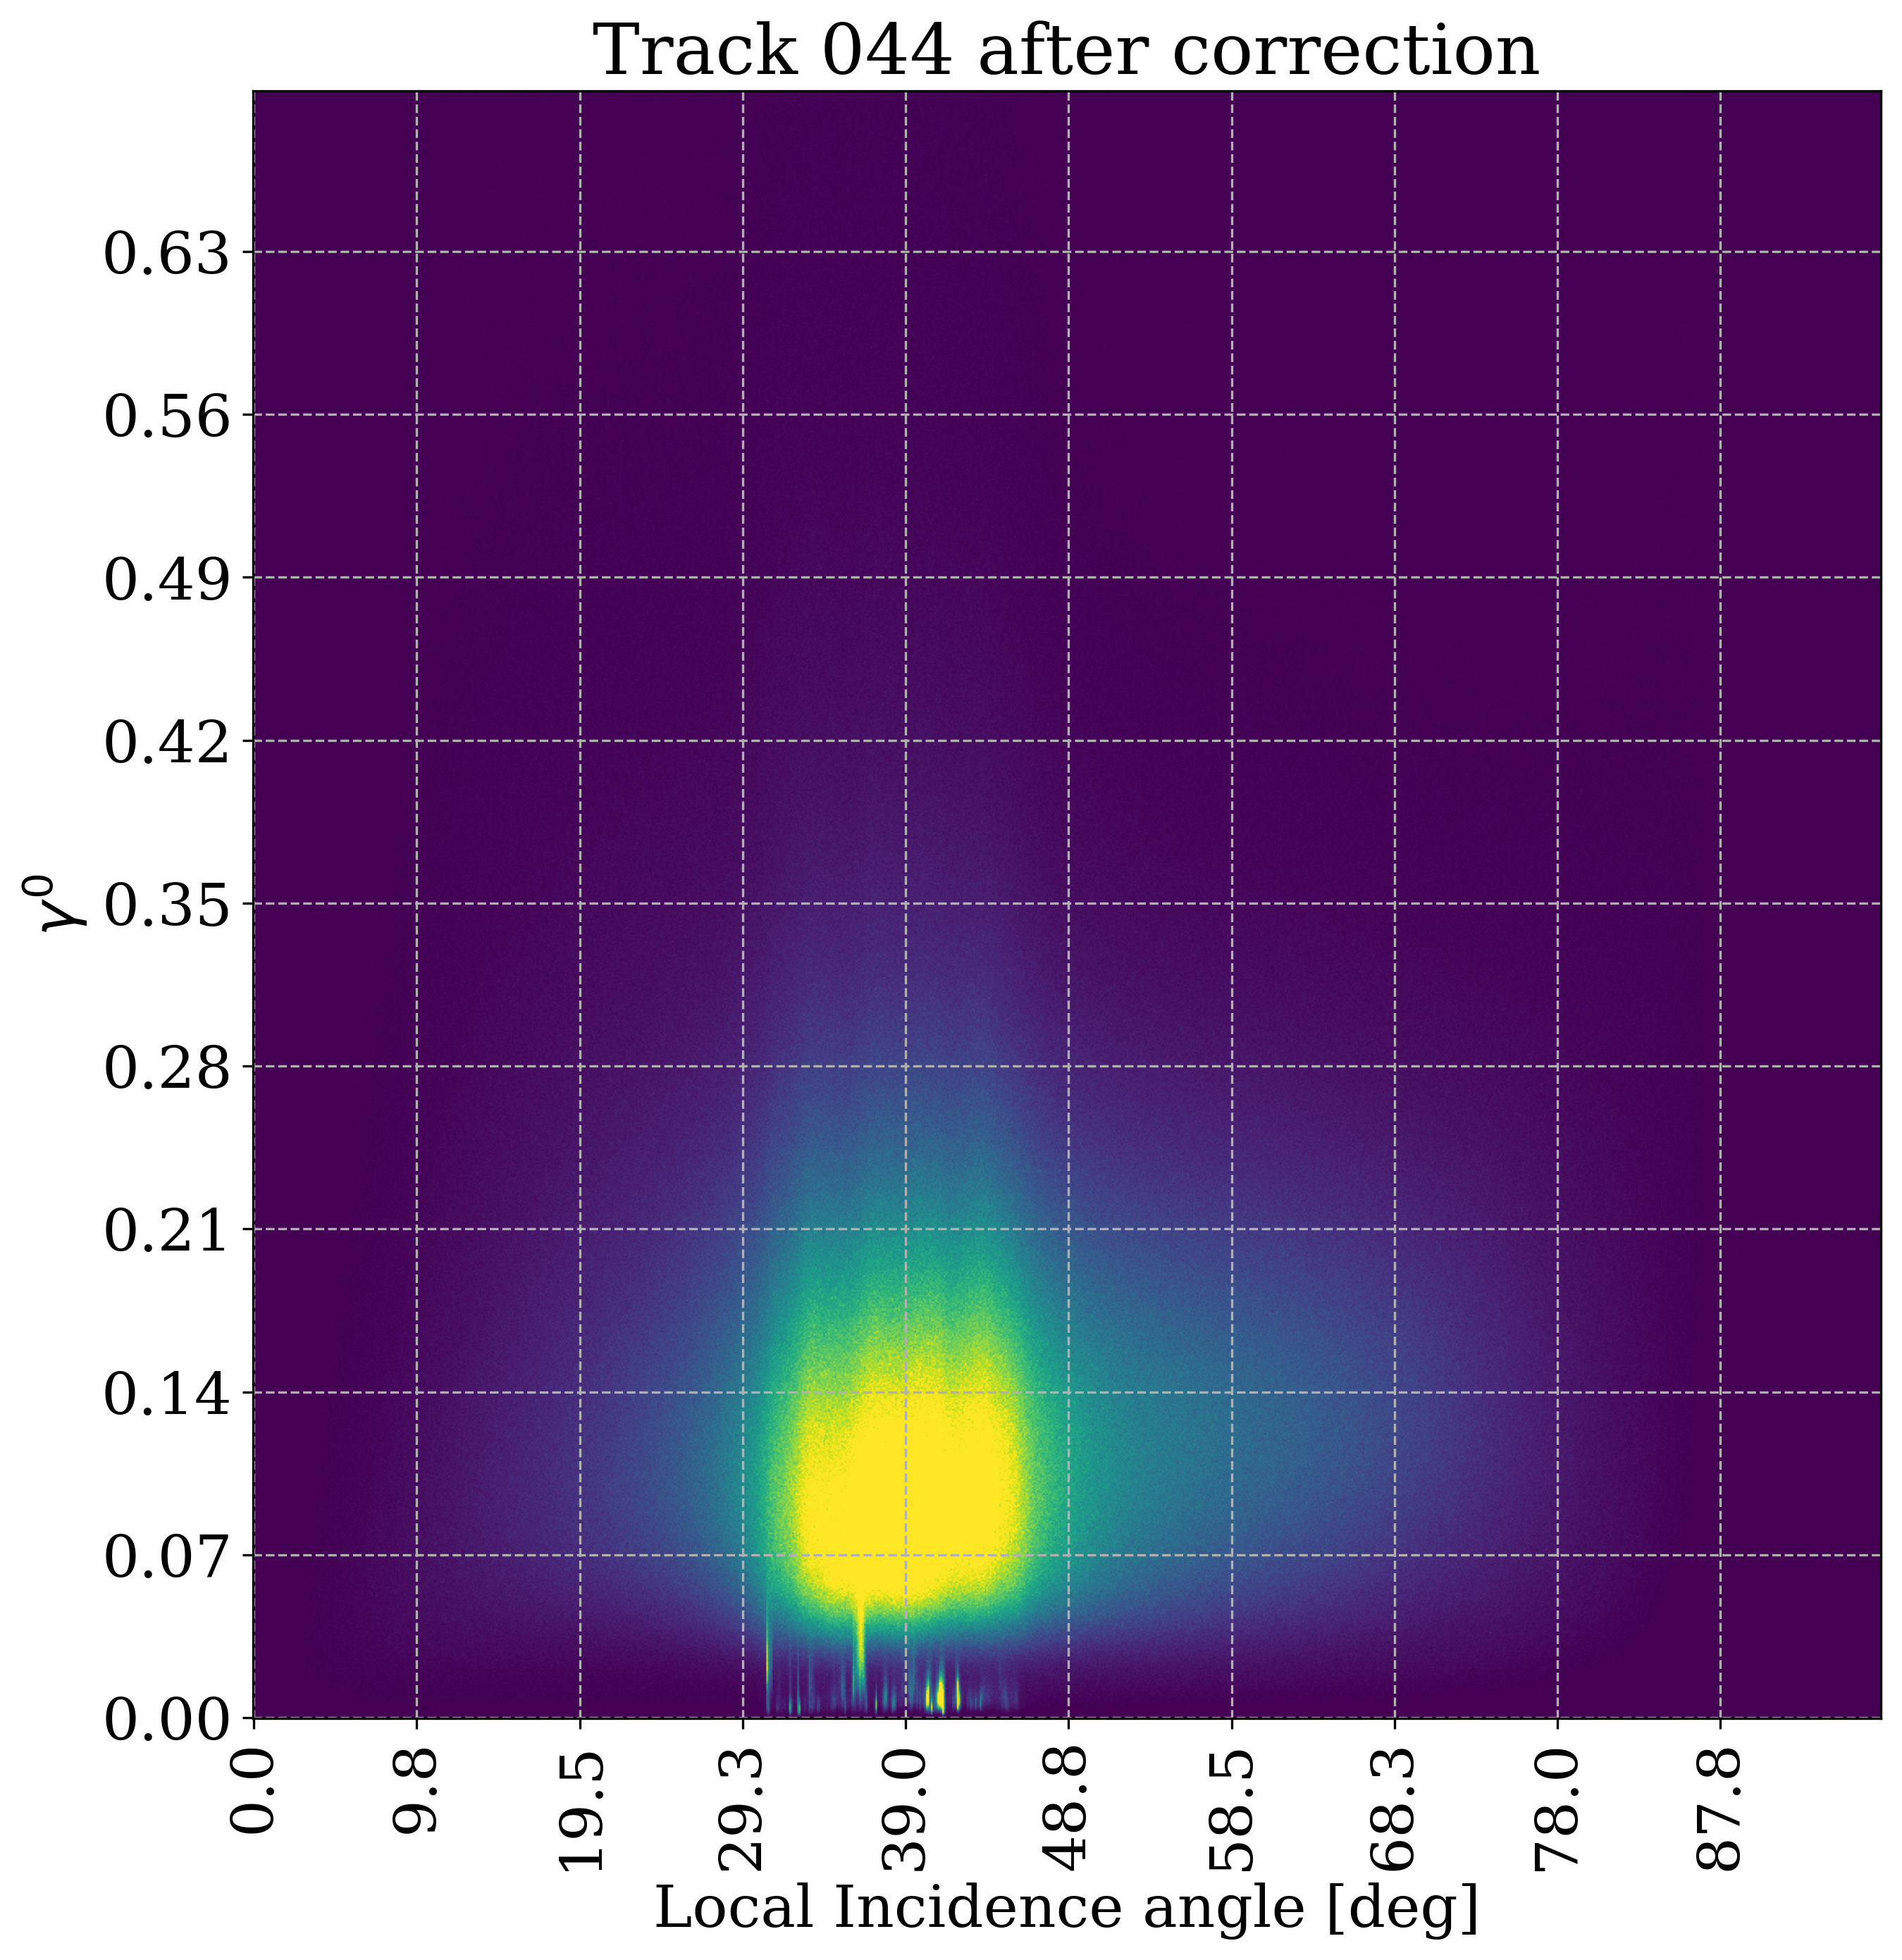
\includegraphics[width=\textwidth]{Figures/nrb/hist_2d_corr.png}
    \caption{}
    \label{fig:hist_2d_corr}
  \end{subfigure}
  \caption{Two-dimensional histograms of NRB versus local slope angle before (a) and after (b) applying the \acs{anf} correction.}
  \label{fig:due_subfigure}
\end{figure}

To further quantify this improvement, we divided the study area into non overlapping patches of size $1000\times1000$ pixels and computed the Pearson correlation coefficient between mean NRB and mean slope angle in each patch. Figure~\ref{fig:correlation_salzburg} plots these coefficients for Sentinel-1 tracks 044 (ascending) and 095 (descending) over Salzburg. Yellow squares correspond to uncorrected data, with correlation values mostly between 0.1 and 0.5. Red circles show the flattened products, where nearly all correlations cluster around zero—confirming the slope compensation step’s ability to eliminate topographically induced radiometric bias.

\begin{figure}[h!]
  \centering
  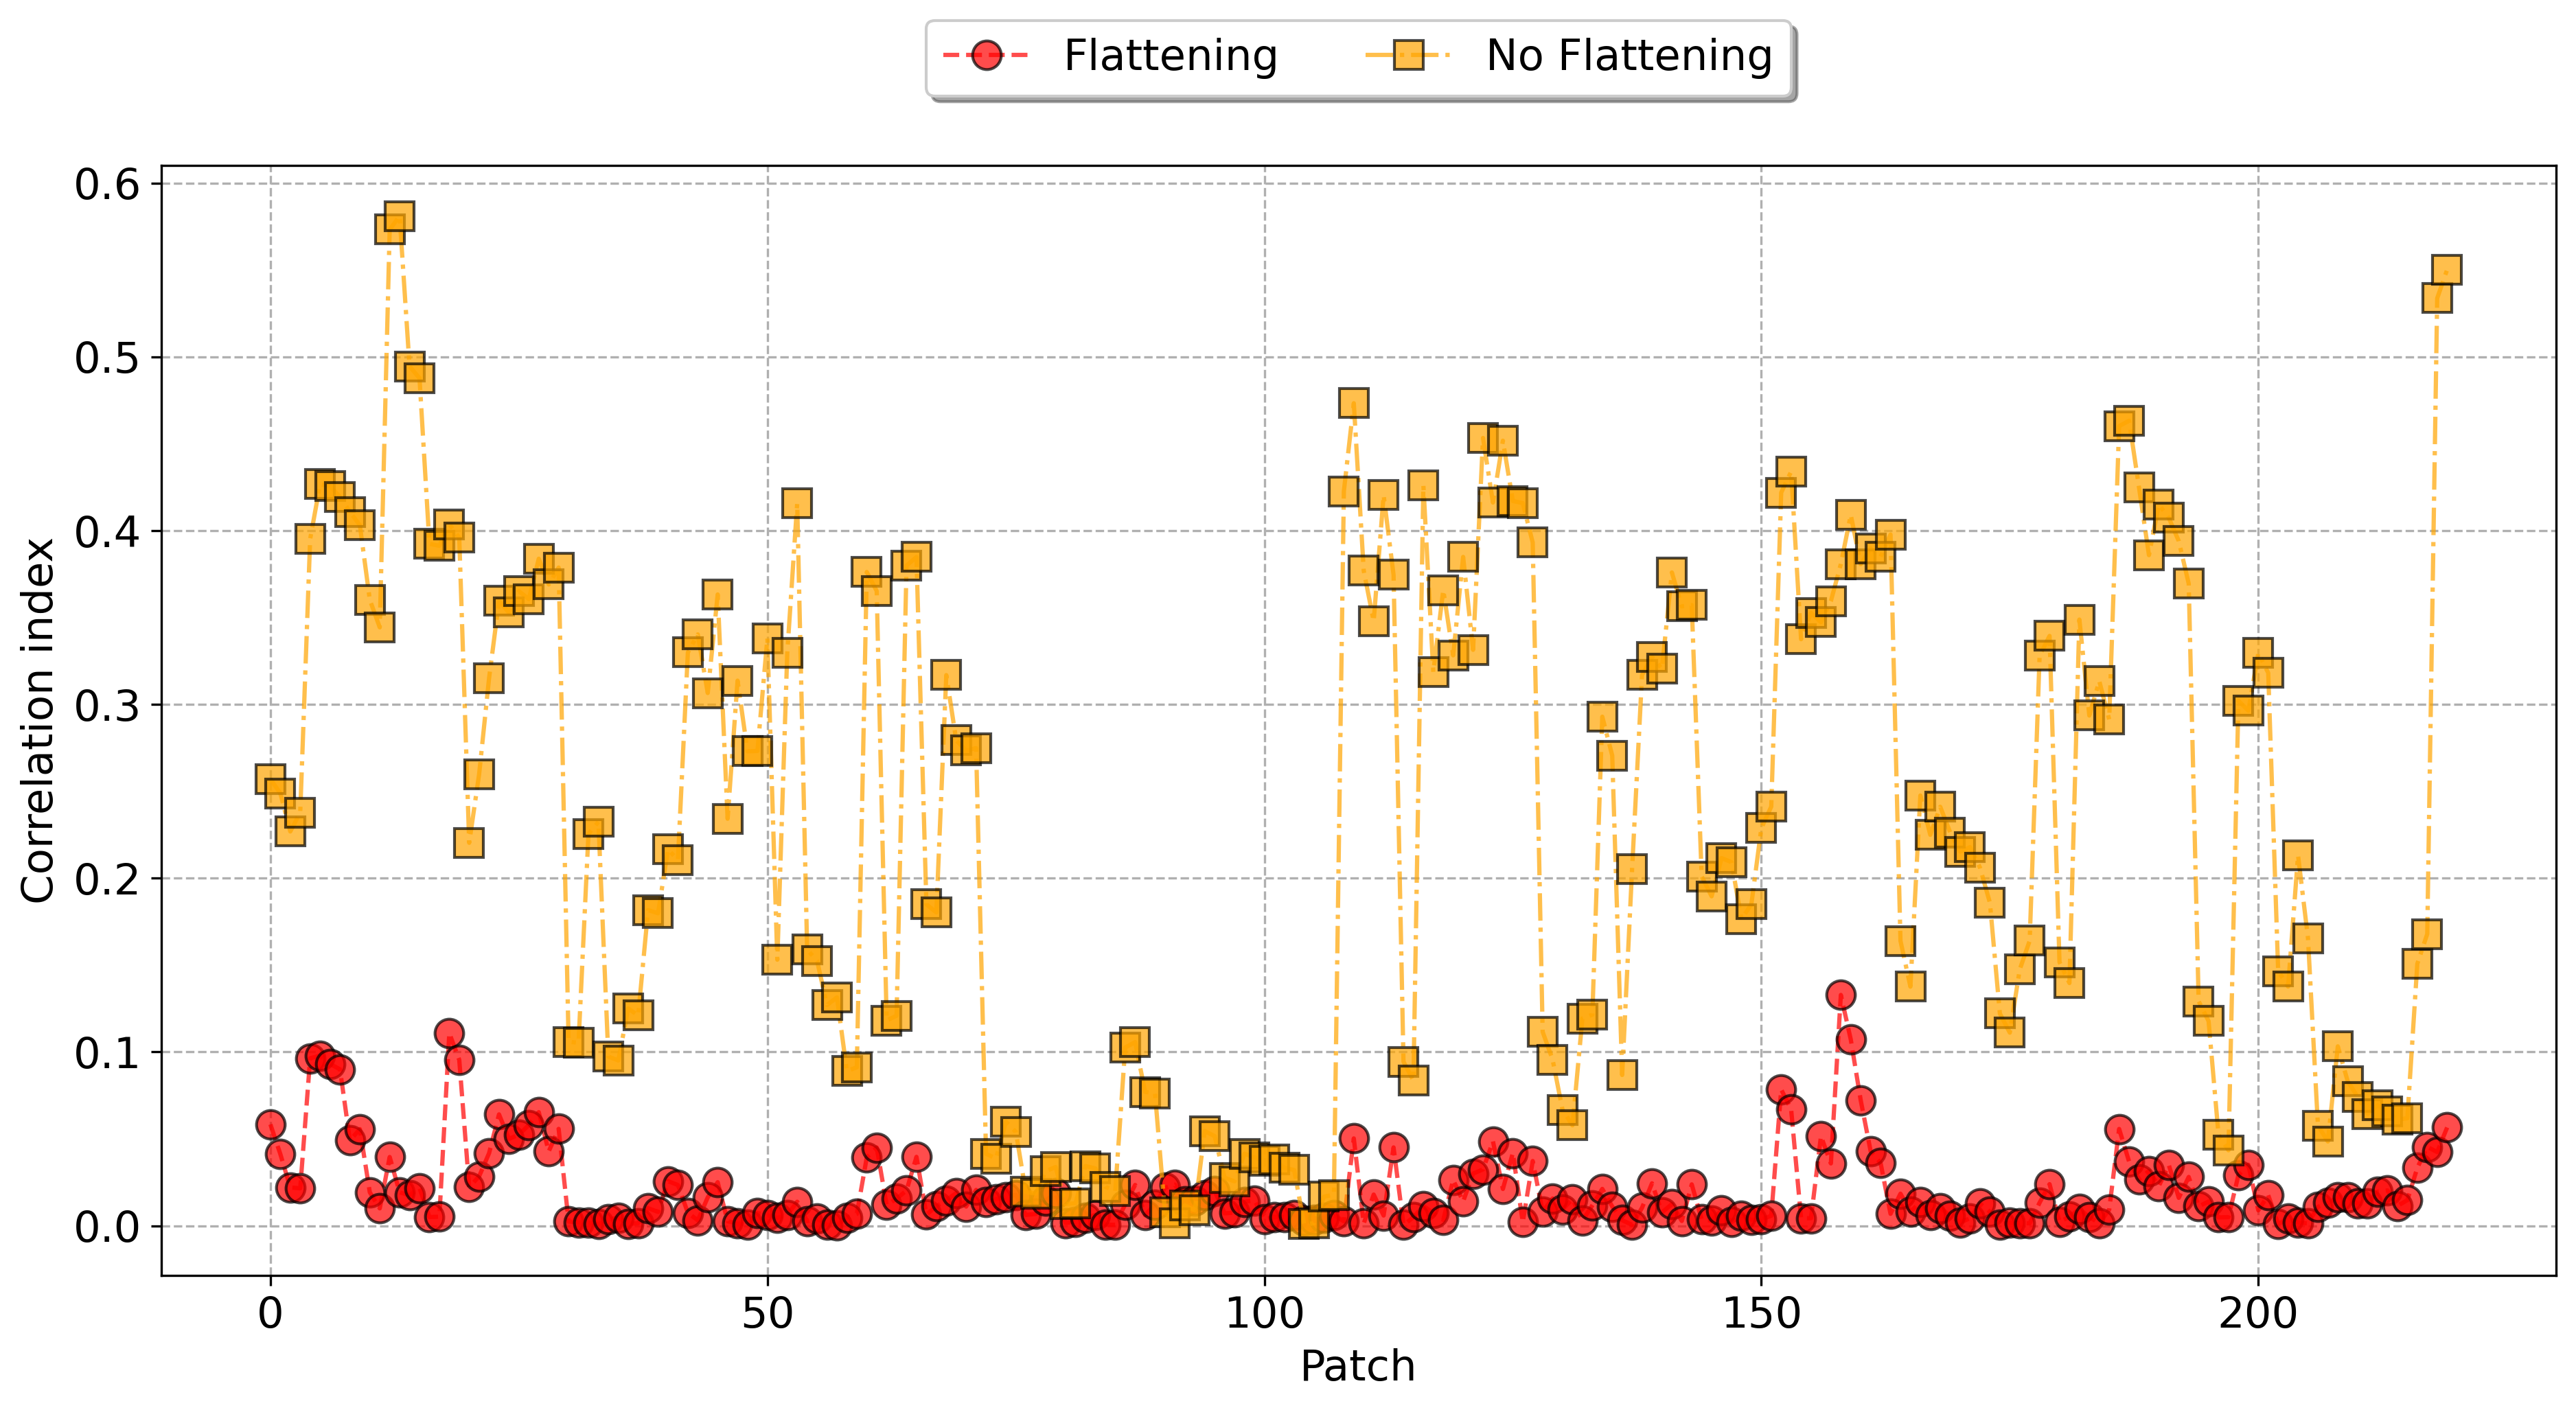
\includegraphics[width=0.9\textwidth]{Figures/nrb/correlation_salzburg.png}
  \caption{Pearson correlation between mean NRB and mean slope angle across $1000\times1000$ pixel patches, before (yellow) and after (red) \acs{anf} correction. Data derive from Sentinel-1 tracks 044 and 095 over Salzburg.}
  \label{fig:correlation_salzburg}
\end{figure}

\paragraph{Slope compensation consistency across acquisition geometries}

We assessed consistency by computing the root mean square difference (RMSD) between ascending and descending acquisitions over identical terrain, as shown in Figure~\ref{fig:rmsd_salzburg}. The analysis used the B-Open S1-RP software on Sentinel-1 IW datasets (tracks 044 and 095) over Salzburg, Austria. Products were first generated at a native 10 m ground resolution; subsequent coarser resolutions (up to 500 m) were obtained via multilooking as described in Section~\ref{sec:nrb_multilook}. 

At the native 10 m resolution, RMSD values range from 3.7 dB to 5.5 dB, dominated by speckle. After multilooking to 500 m, the effect of speckle diminishes markedly, yielding RMSD of about 1.2 dB for the 10 m DEM geogrid and 1.7 dB for the 30 m DEM geogrid. These findings confirm that slope flattening, eventually combined with appropriate multilooking, delivers robust NRB products independent of viewing geometry.

\begin{figure}[h!]
  \centering
  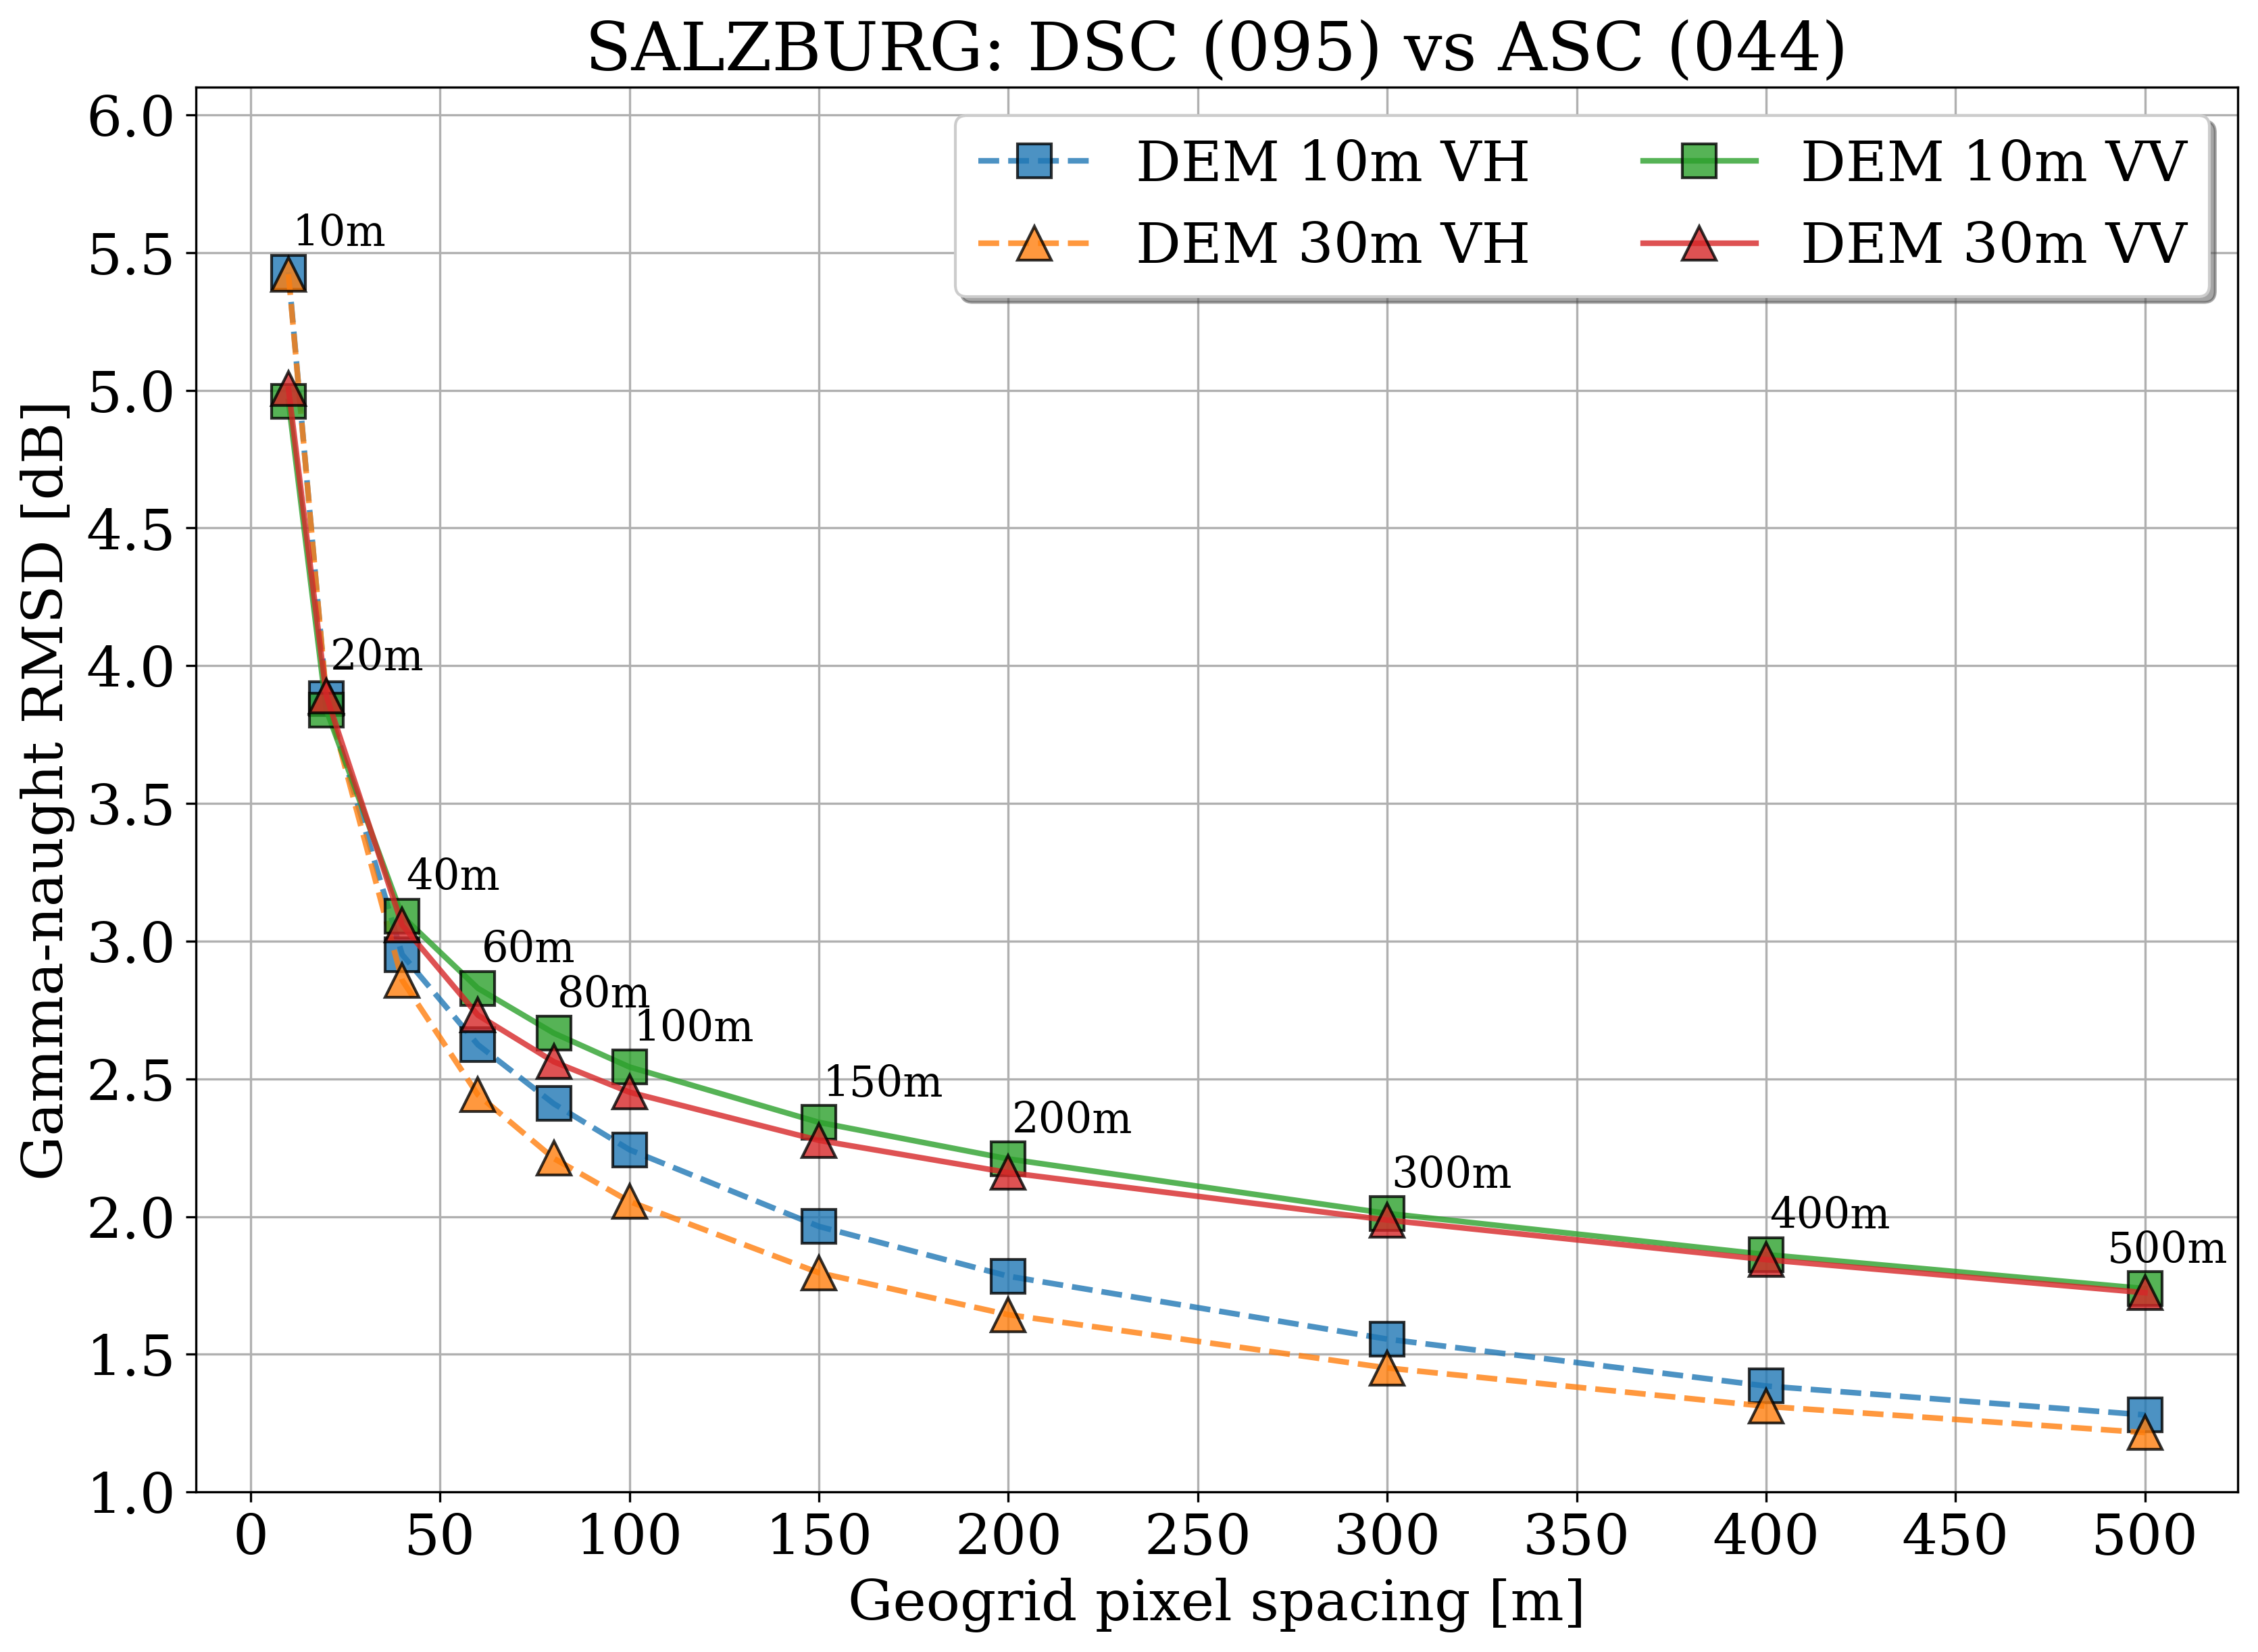
\includegraphics[width=0.9\textwidth]{Figures/nrb/db_with_10m.png}
  \caption{Root mean square difference between ascending and descending NRB products over Salzburg, using DEM geogrids of 10 m and 30 m and multilooked resolutions from 10 m up to 500 m.}
  \label{fig:rmsd_salzburg}
\end{figure}

\subsection{Dependence on External Data}
\label{sec:nrb_dependence_external}

\subsubsection{Dependence on DEM Resolution and Quality}

The accuracy of radiometric terrain correction in complex terrain relies critically on the resolution and vertical accuracy of the Digital Elevation Model (DEM). A high resolution DEM captures local slope variations and terrain morphology more precisely, enabling more accurate estimation of the local incidence angle and illuminated ground area. Conversely, coarser or error-prone DEMs smooth out fine scale slopes and introduce biases in the computed Area Normalization Factor (ANF), which in turn degrade the quality of the generated NRB product.

\paragraph{Theoretical model}
\label{sec:nrb_theoretical_model_dem}

For a single DEM facet the ANF is defined as the projection of a slant range pixel’s ground footprint onto a plane orthogonal to the sensor’s line of sight. Let \(A\) be the true ground cell area and \(\theta_i\) the local incidence angle (the angle between the radar line of sight and the normal to the DEM facet). Then
\begin{equation}
  \label{eq:ANF}
  \gamma_{\mathrm{ANF}} \;=\; A \,\cos\!\theta_i.
\end{equation}

Considering that multiple DEM facets can partially contribute to the same radar cell, let \(j\) be the index of the DEM facet, let \(l\) be the index of the radar cell, let \(J(l)\) the set of DEM facets covering the radar cell \(l\), let \(w_{j,l}\) the percentage of coverage of the radar cell \(l\) by the DEM facet \(j\), the ANF associate to the radar cell is given by:

\begin{equation}
  \label{eq:ANF_integral}
  \gamma_{\mathrm{ANF}_l} = \sum_{j \in J(l)} A_j w_{j,l} \cos\!\theta_{i_j} \,\bigl(1 - \delta\theta_{i_j} \tan\!\theta_{i_j}\bigr).
\end{equation}

In order to simplify the equation and evaluate the error on the ANF it is possible to identify an upper-bound for the local incidence angle and the value of \(\delta\theta\).

If the DEM has an elevation error \(\sigma_h\), this propagates into an incidence angle error \(\delta\theta_i\approx \sigma_h / dx\), where \(dx\) is the horizontal DEM sampling. A first order Taylor expansion of \eqref{eq:ANF} yields
\begin{equation}
  \label{eq:ANF_first_ord}
  |\Delta \gamma_{\mathrm{ANF}_l}| \le \sum_{j \in J(l)} A_j w_{j,l} \cos\!\theta_{i_j} \,\bigl(\delta\theta_{\mathrm{max}} \tan\!\theta_{\mathrm{max}}\bigr) = \gamma_{\mathrm{ANF}_l} \bigl(\delta\theta_{\mathrm{max}} \tan\!\theta_{\mathrm{max}}\bigr).
\end{equation}
Thus, the variance of the ANF error due to DEM noise is
\begin{equation}
  \sigma^2_{\gamma_{\mathrm{ANF}_h}}
  = \gamma^2_{\mathrm{ANF}}
    \Bigl(\tfrac{\tan\!\theta_{\mathrm{max}}}{dx}\Bigr)^{\!2}\,\sigma^2_h.
\end{equation}
This expression shows that DEM errors have the greatest impact where the slope (and hence \(\tan\theta_{\mathrm{max}}\)) is large, and diminish as the DEM pixel size \(dx\) increases.

\paragraph{Test on real data}

To quantify this effect, we computed the ANF over a steep alpine test area using two Copernicus DEMs sampled at \(10\) m and \(30\) m. We then evaluated the ratio in dB between the two ANFs:
\[
  \Delta_{\mathrm{ANF}}(\mathrm{dB})
  = 10\log_{10}\!\bigl(\gamma_{\mathrm{ANF}}^{10\mathrm{m}} / \gamma_{\mathrm{ANF}}^{30\mathrm{m}}\bigr).
\]
Figure~\ref{fig:ANF_DIFF_DB_DEM} maps this difference. As predicted by \eqref{eq:ANF_first_ord}, the largest deviations (up to \(1\)\,dB) occur on the steepest slopes. Smaller but not negligible differences also appear over urban or flat terrain where fine scale surface features are not captured by the coarser DEM.

\begin{figure}[h!]
  \centering
  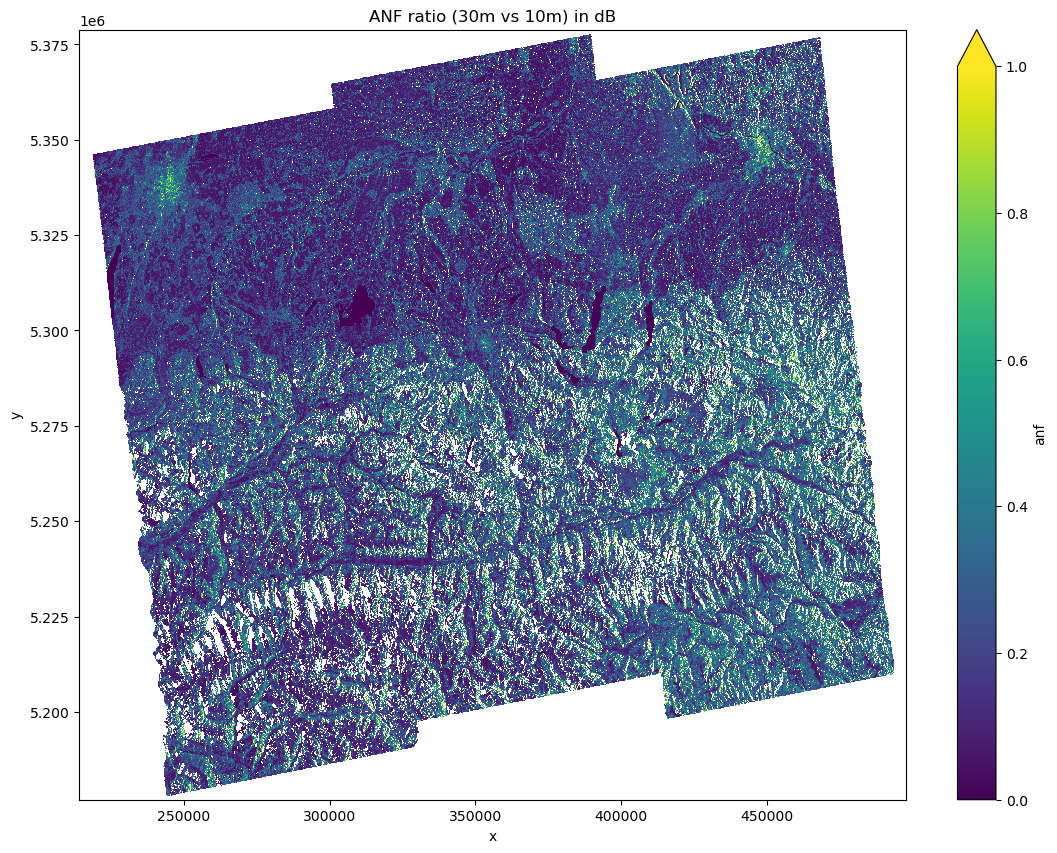
\includegraphics[width=0.9\textwidth]{Figures/nrb/anf_ratio_10m_vs_30m_dem.png}
  \caption{Difference in ANF (dB) between 10 m and 30 m DEMs. Larger deviations align with steep slopes, consistent with the first order model in \eqref{eq:ANF_first_ord}.}
  \label{fig:ANF_DIFF_DB_DEM}
\end{figure}

This comparison highlights spatial patterns of ANF error but does not identify which DEM yields the best NRB product. Definitive assessment requires radiometric analysis of actual SAR data acquired under multiple geometries (see Section~\ref{sec:nrb_stability_diff_geom}). At full resolution, speckle and image variability dominate these differences. Applying multilooking mitigates this issue, however at coarser resolutions the remaining differences are minor, serving mainly to reveal systematic bias.

\subsubsection{Slope Correction (ANF) and Orbital Tube Control}

The ANF also depends on the sensor’s precise position and attitude, which vary within the orbital tube. Even small deviations in the satellite’s orbit introduce errors in slant range geometry and thus in the computed incidence angle. Because Sentinel-1’s orbital tube is on the order of few hundreds of meters, the resulting ANF variations are relatively small, and in practice one can compute a single flattening layer for the nominal track and apply it to all scenes.

\paragraph{Theoretical model}
\label{sec:nrb_theoretical_model_orbital}

If an across-track baseline error \(B_{\perp}\) shifts the sensor off the nominal orbit, the resulting incidence angle perturbation is \(\delta\theta_i \approx B_{\perp}/R\), where \(R\) is the slant range distance. Starting from \eqref{eq:ANF_integral}, the corresponding ANF variation is
\begin{equation}
  \label{eq:ANF_first_ord_B_perp}
  \gamma_{\mathrm{ANF}_l}' 
  = \sum_{j \in J(l)} A_j w_{j,l} \cos\!\theta_{i_j} \,\bigl(1 - \tfrac{B_{\perp}}{R} \tan\!\theta_{i_j}\bigr),
\end{equation}
and its variance becomes
\begin{equation}
  \sigma^2_{\gamma_{\mathrm{ANF}_{B_\perp}}}
  = \gamma^2_{\mathrm{ANF}}
    \Bigl(\tfrac{\tan\!\theta_{\mathrm{max}}}{R}\Bigr)^{\!2}\,\sigma^2_{B_{\perp}}.
\end{equation}
Since \(R/dx\gg1\), DEM induced ANF errors dominate over orbital tube errors. Equation~\eqref{eq:ANF_first_ord_B_perp} also shows that a simple scaling, dependent on the angle, of the nominal ANF compensates for baseline variations up to a few kilometers.

\paragraph{Test on real data}

We validated these predictions using a stack of SAOCOM acquisitions over Naples, where the interferometric perpendicular baseline spans several kilometers. For each orbit realization, we computed the ground geometry ANF (no SAR image content involved) and then derived its spatial standard deviation. Figure~\ref{fig:ANF_STD_NAPLES} plots the measured \(\sigma_{\mathrm{ANF}}\): as expected, a correlation with the terrain slope is clearly visible: the variability of the ANF increases with slope, but in any case its variation is very small. The corresponding mean ANF across orbits is shown in Figure~\ref{fig:ANF_MEAN_NAPLES}.
Figure~\ref{fig:ANF_HISTOGRAM} shows a histogram of the maximum and minimum $ANF/ANF_{mean}$ ratios, which form two extremely narrow distributions, within $0.02$ dB.
\begin{figure}[h!]
  \centering
  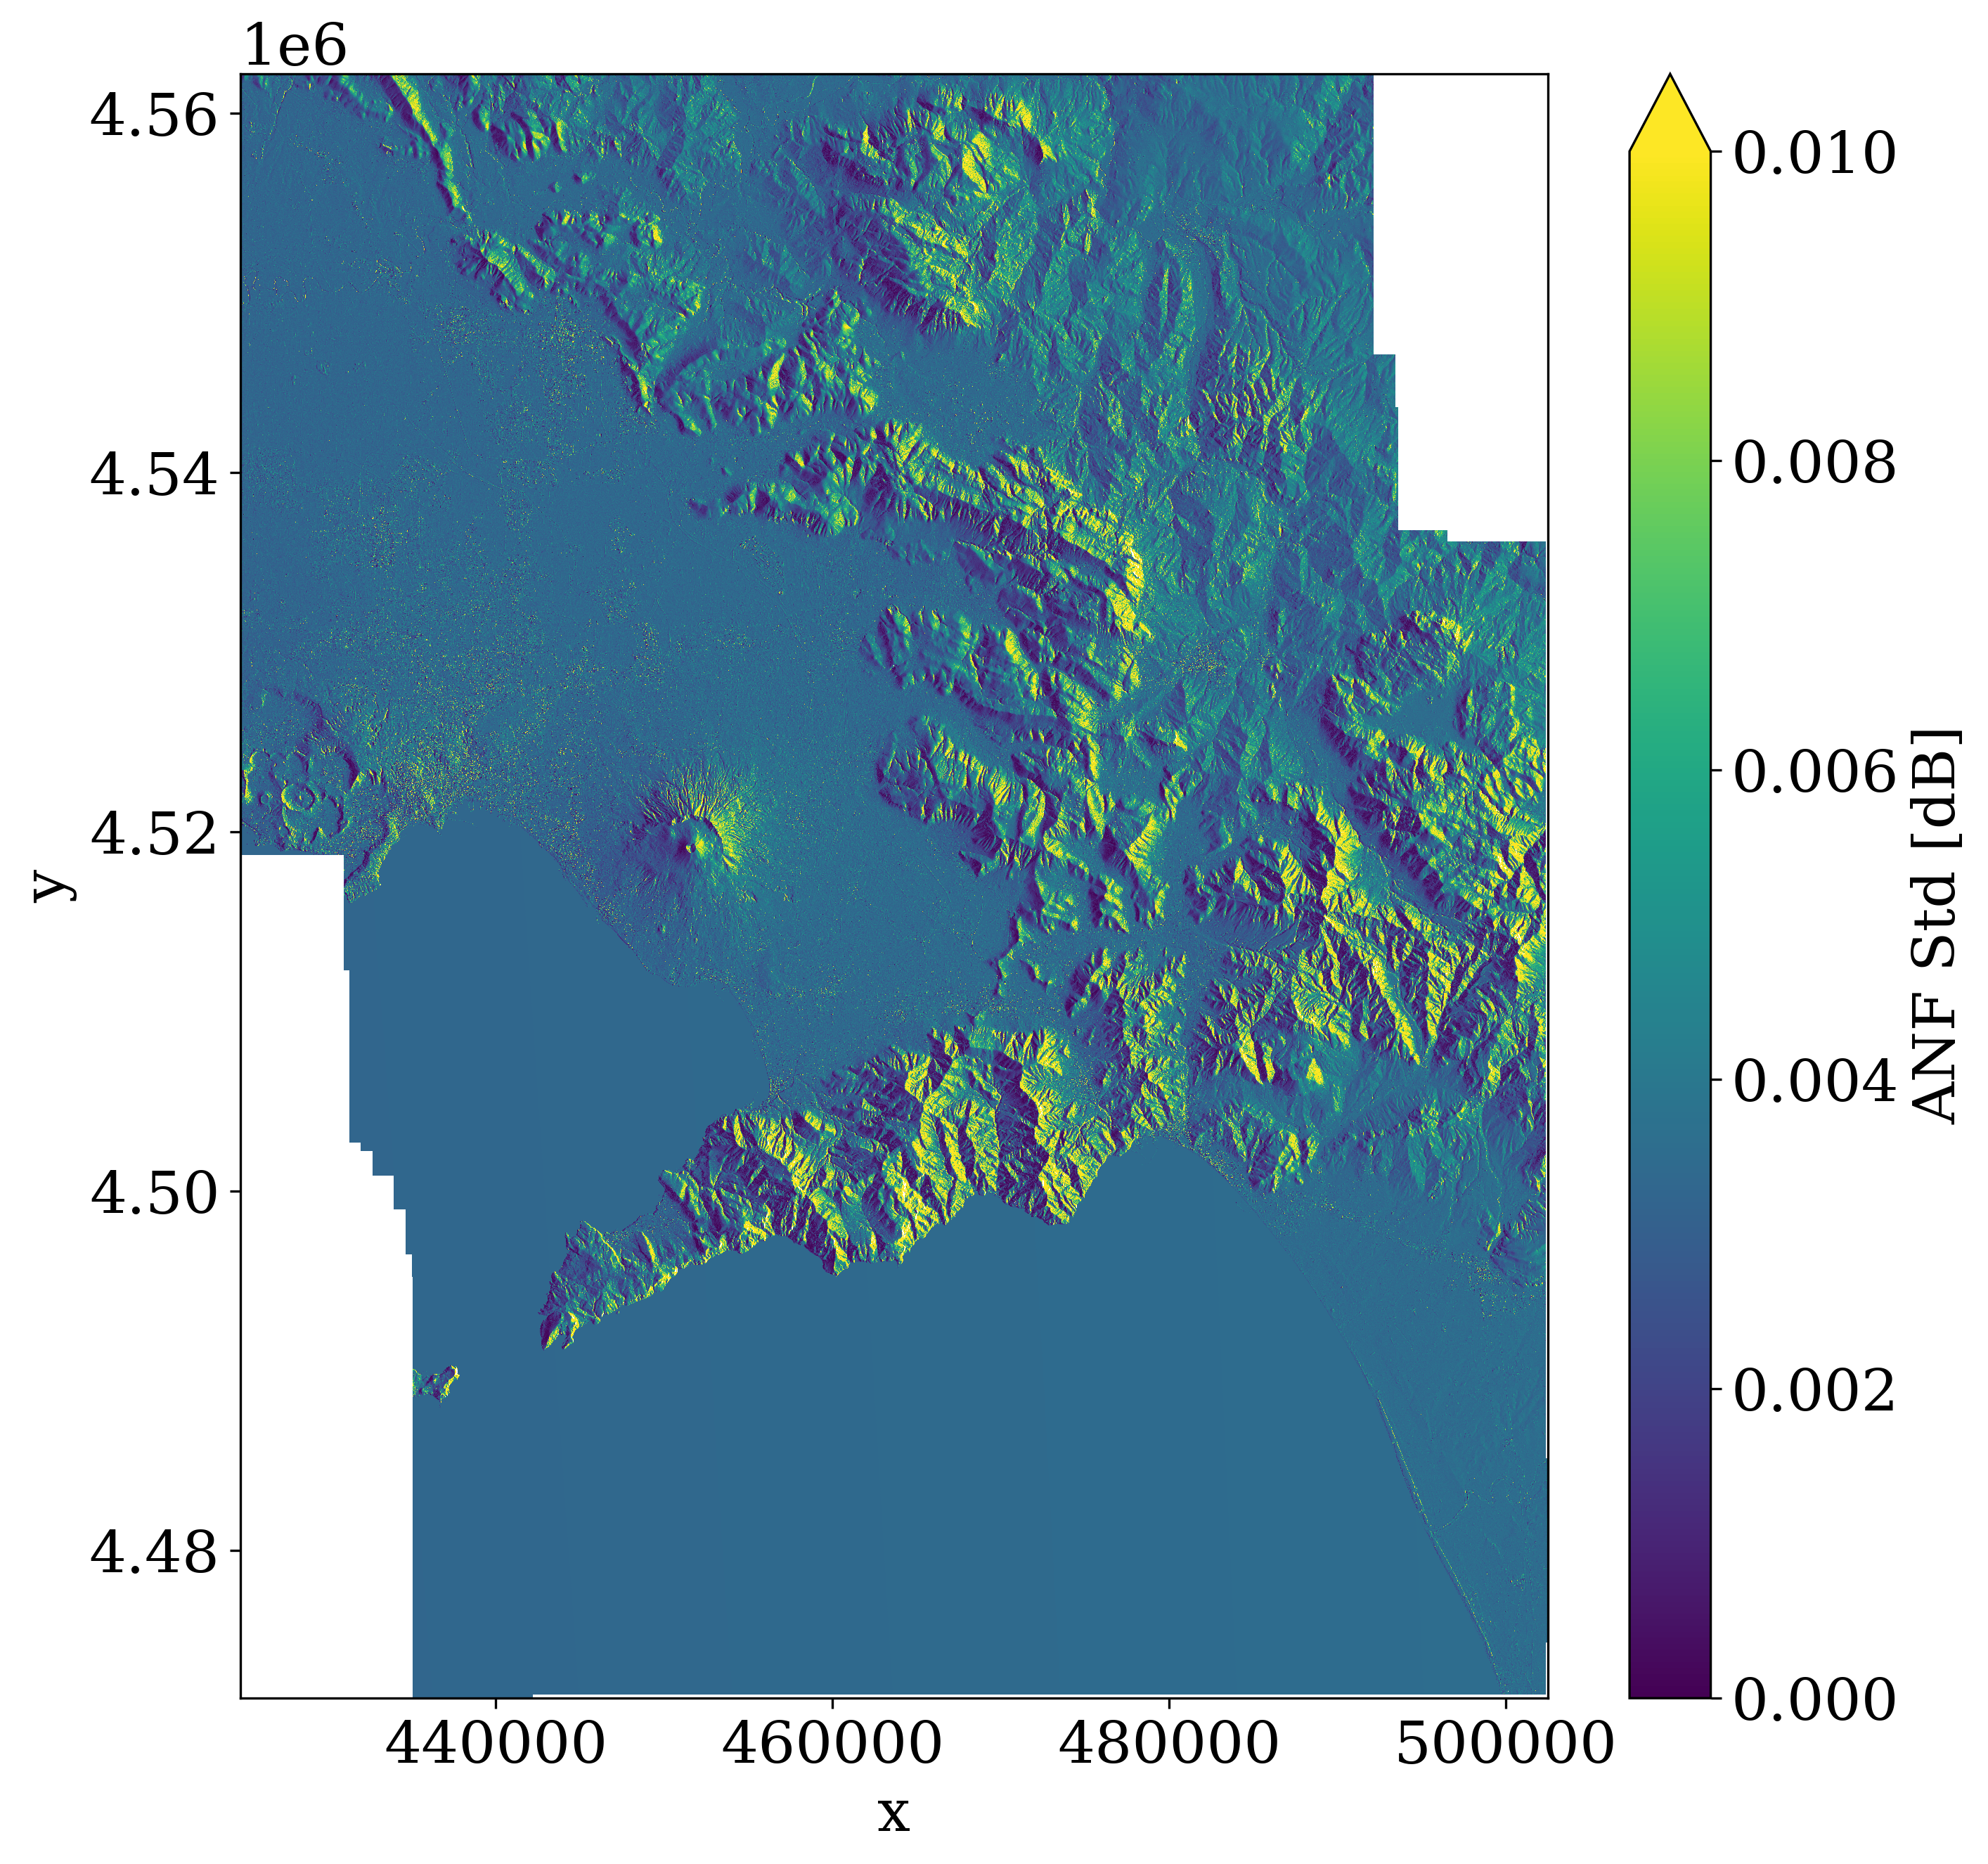
\includegraphics[width=0.9\textwidth]{Figures/nrb/anf_std_NAPLES.png}
  \caption{Standard deviation of ANF across multiple SAOCOM orbits over Naples. The image clearly shows that the ANF Variability increases with slope, in agreement with \eqref{eq:ANF_first_ord_B_perp}.}
  \label{fig:ANF_STD_NAPLES}
\end{figure}

\begin{figure}[h!]
  \centering
  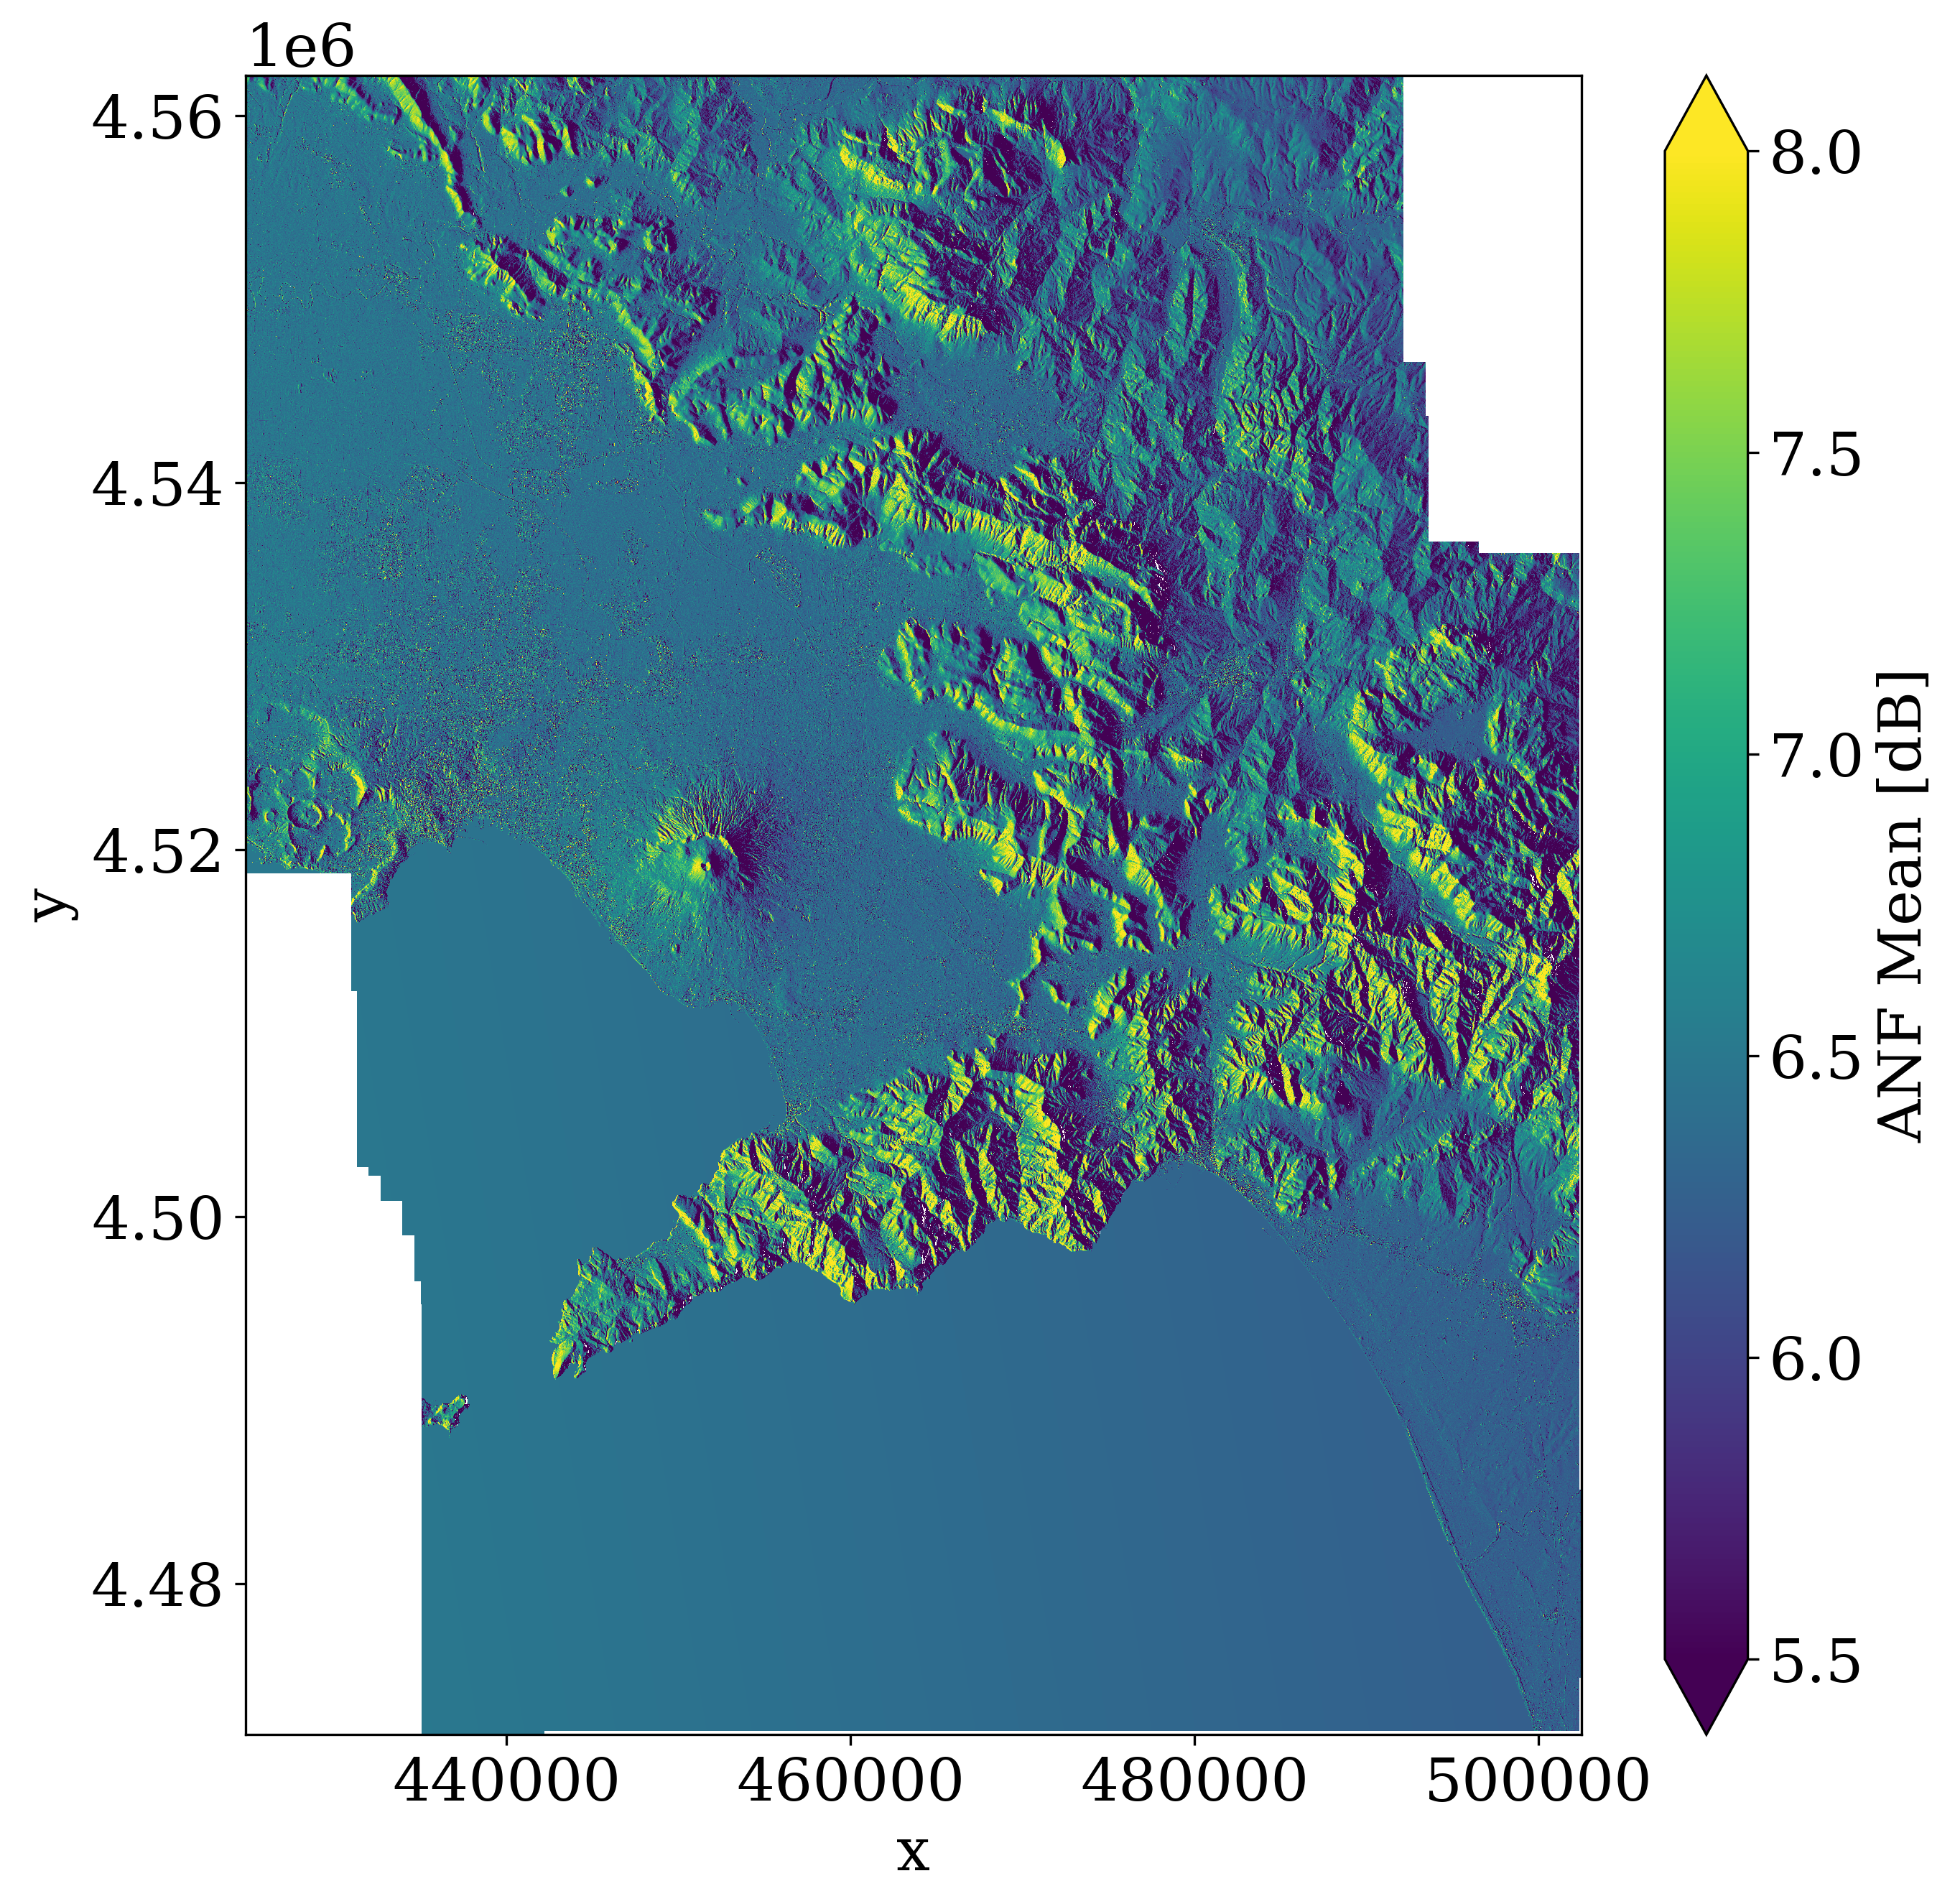
\includegraphics[width=0.9\textwidth]{Figures/nrb/anf_mean_NAPLES.png}
  \caption{Mean ANF across SAOCOM orbit realizations over Naples. The gradient reflects the cosine dependence in \eqref{eq:ANF}.}
  \label{fig:ANF_MEAN_NAPLES}
\end{figure}

\begin{figure}[h!]
  \centering
  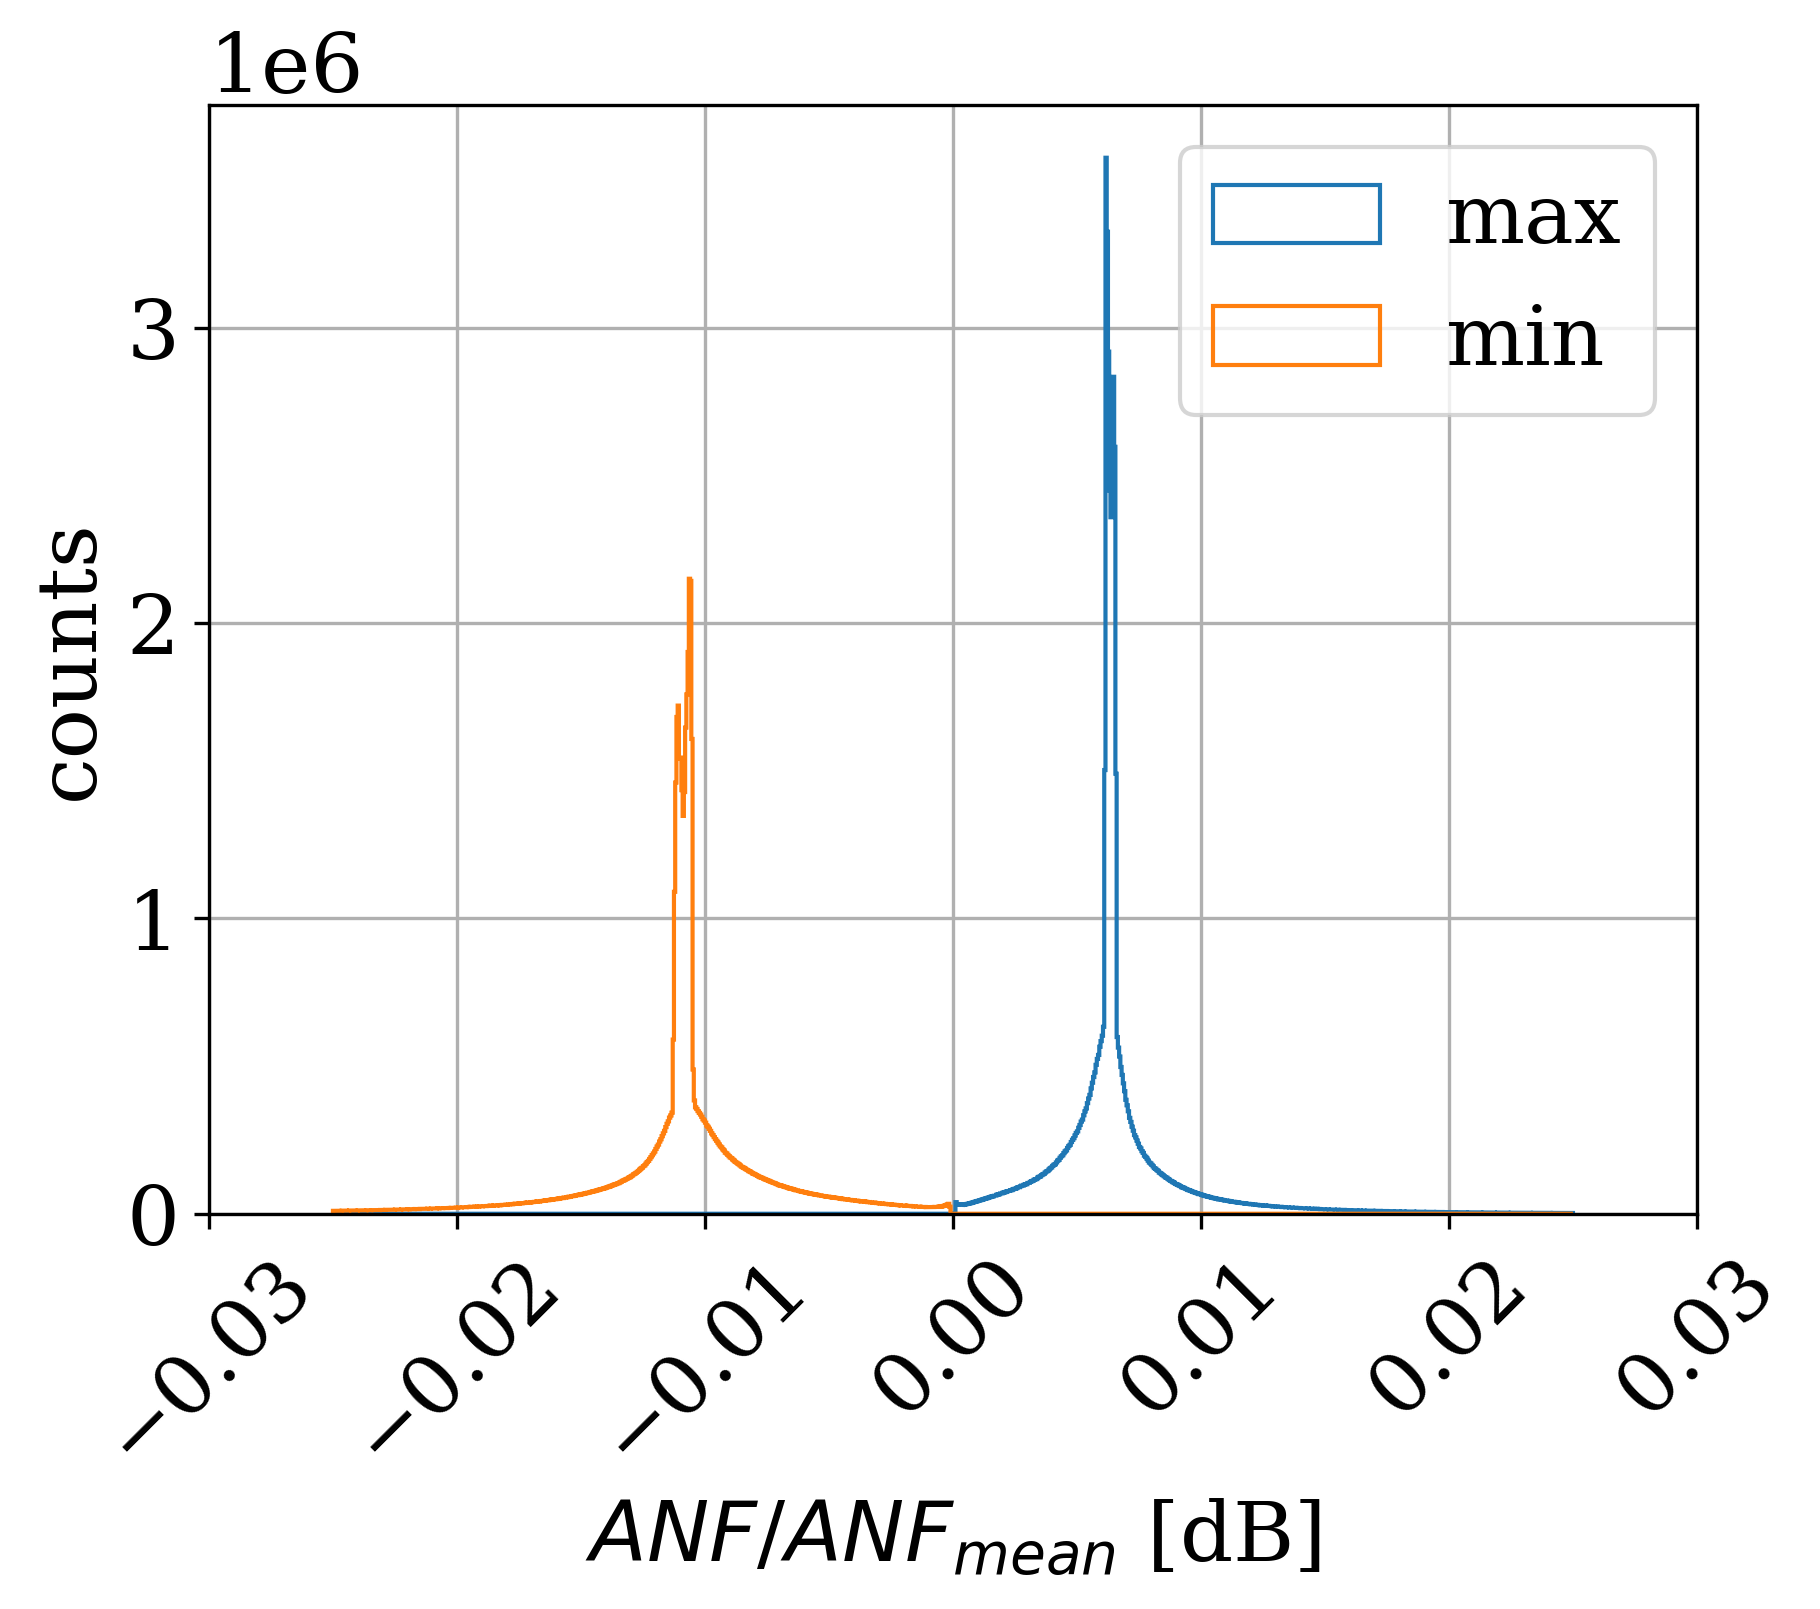
\includegraphics[width=0.9\textwidth]{Figures/nrb/histogram_ANF.png}
  \caption{Histogram of the maximum and minimum $ANF/ANF_{mean}$ ratio from SAOCOM orbit realizations over Naples. Both distributions are extremely narrow, within $0.02$ dB, indicating very low variance.}
  \label{fig:ANF_HISTOGRAM}
\end{figure}


Figure~\ref{fig:ANF_VS_BAS} shows the spatially averaged relative ANF (\(\Delta\mathrm{ANF}\)) versus \(|B_{\perp}|\). The near linear trend confirms the analytic scaling in \eqref{eq:ANF_first_ord_B_perp}, and even for baselines of 1 km the relative ANF error remains below 0.1 dB. Finally, Figure~\ref{fig:ANF_VS_INC_ANGLE} presents a two-dimensional scatter plot of ANF variability against incidence angle, with the theoretical first order curve overlaid. The close match validates our analytic model and suggests that a single, precomputed slope flattening layer, properly rescaled, suffices for an entire satellite track.

\begin{figure}[h!]
  \centering
  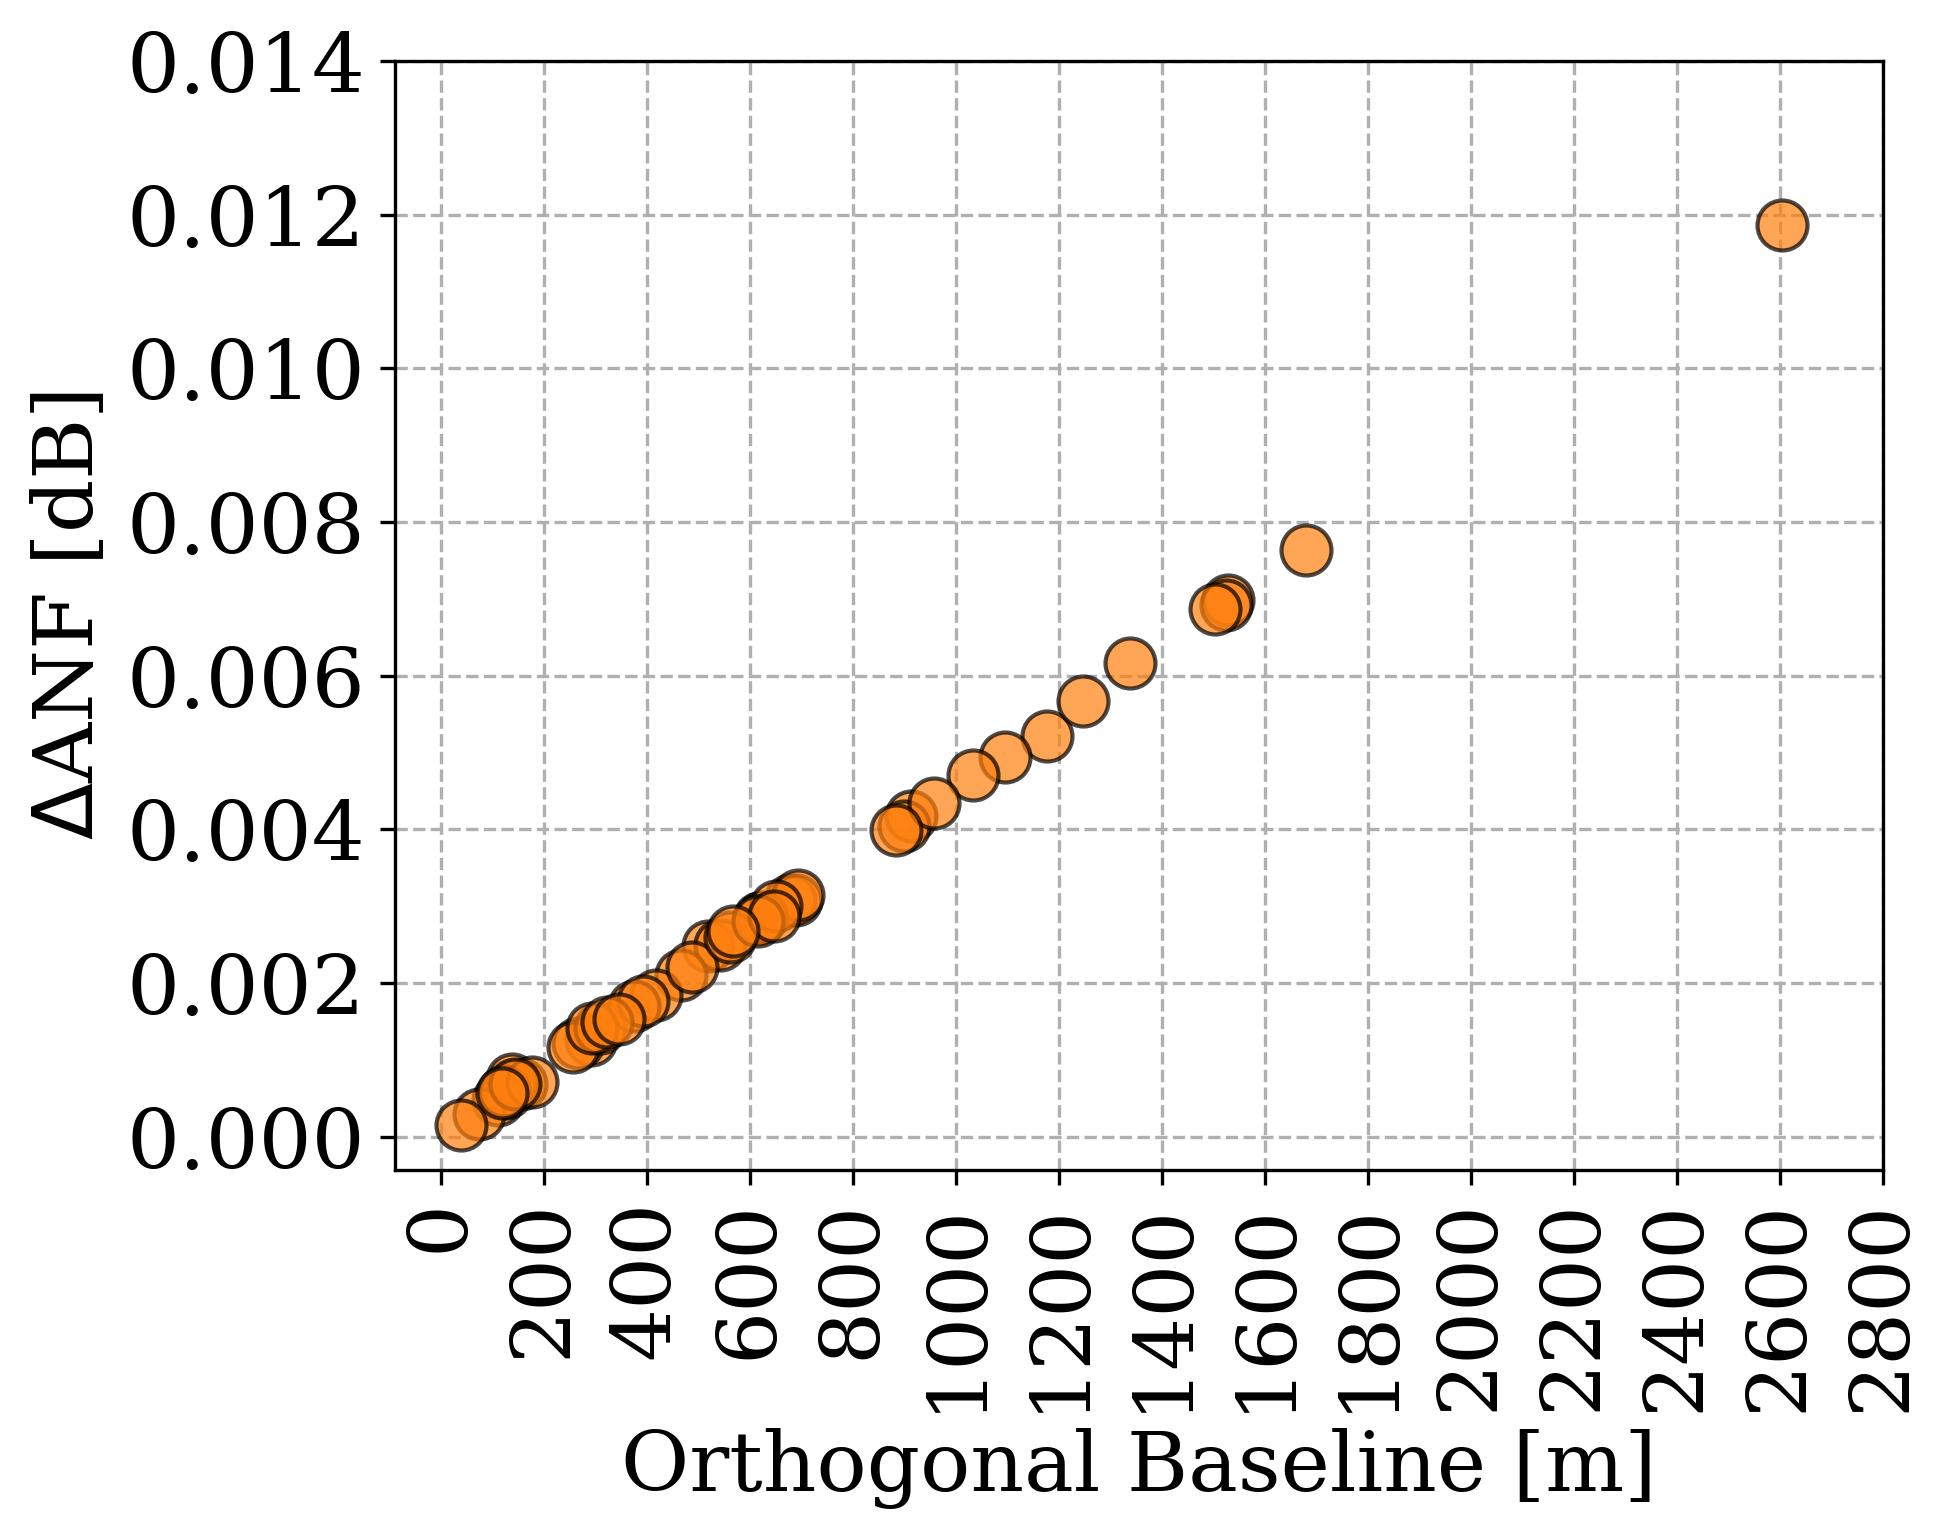
\includegraphics[width=0.9\textwidth]{Figures/nrb/baseline_division.png}
  \caption{Spatial average of \(\Delta\mathrm{ANF}\) versus the absolute perpendicular baseline \(|B_{\perp}|\). The linear increase matches the prediction of \eqref{eq:ANF_first_ord_B_perp}.}
  \label{fig:ANF_VS_BAS}
\end{figure}

\begin{figure}[h!]
  \centering
  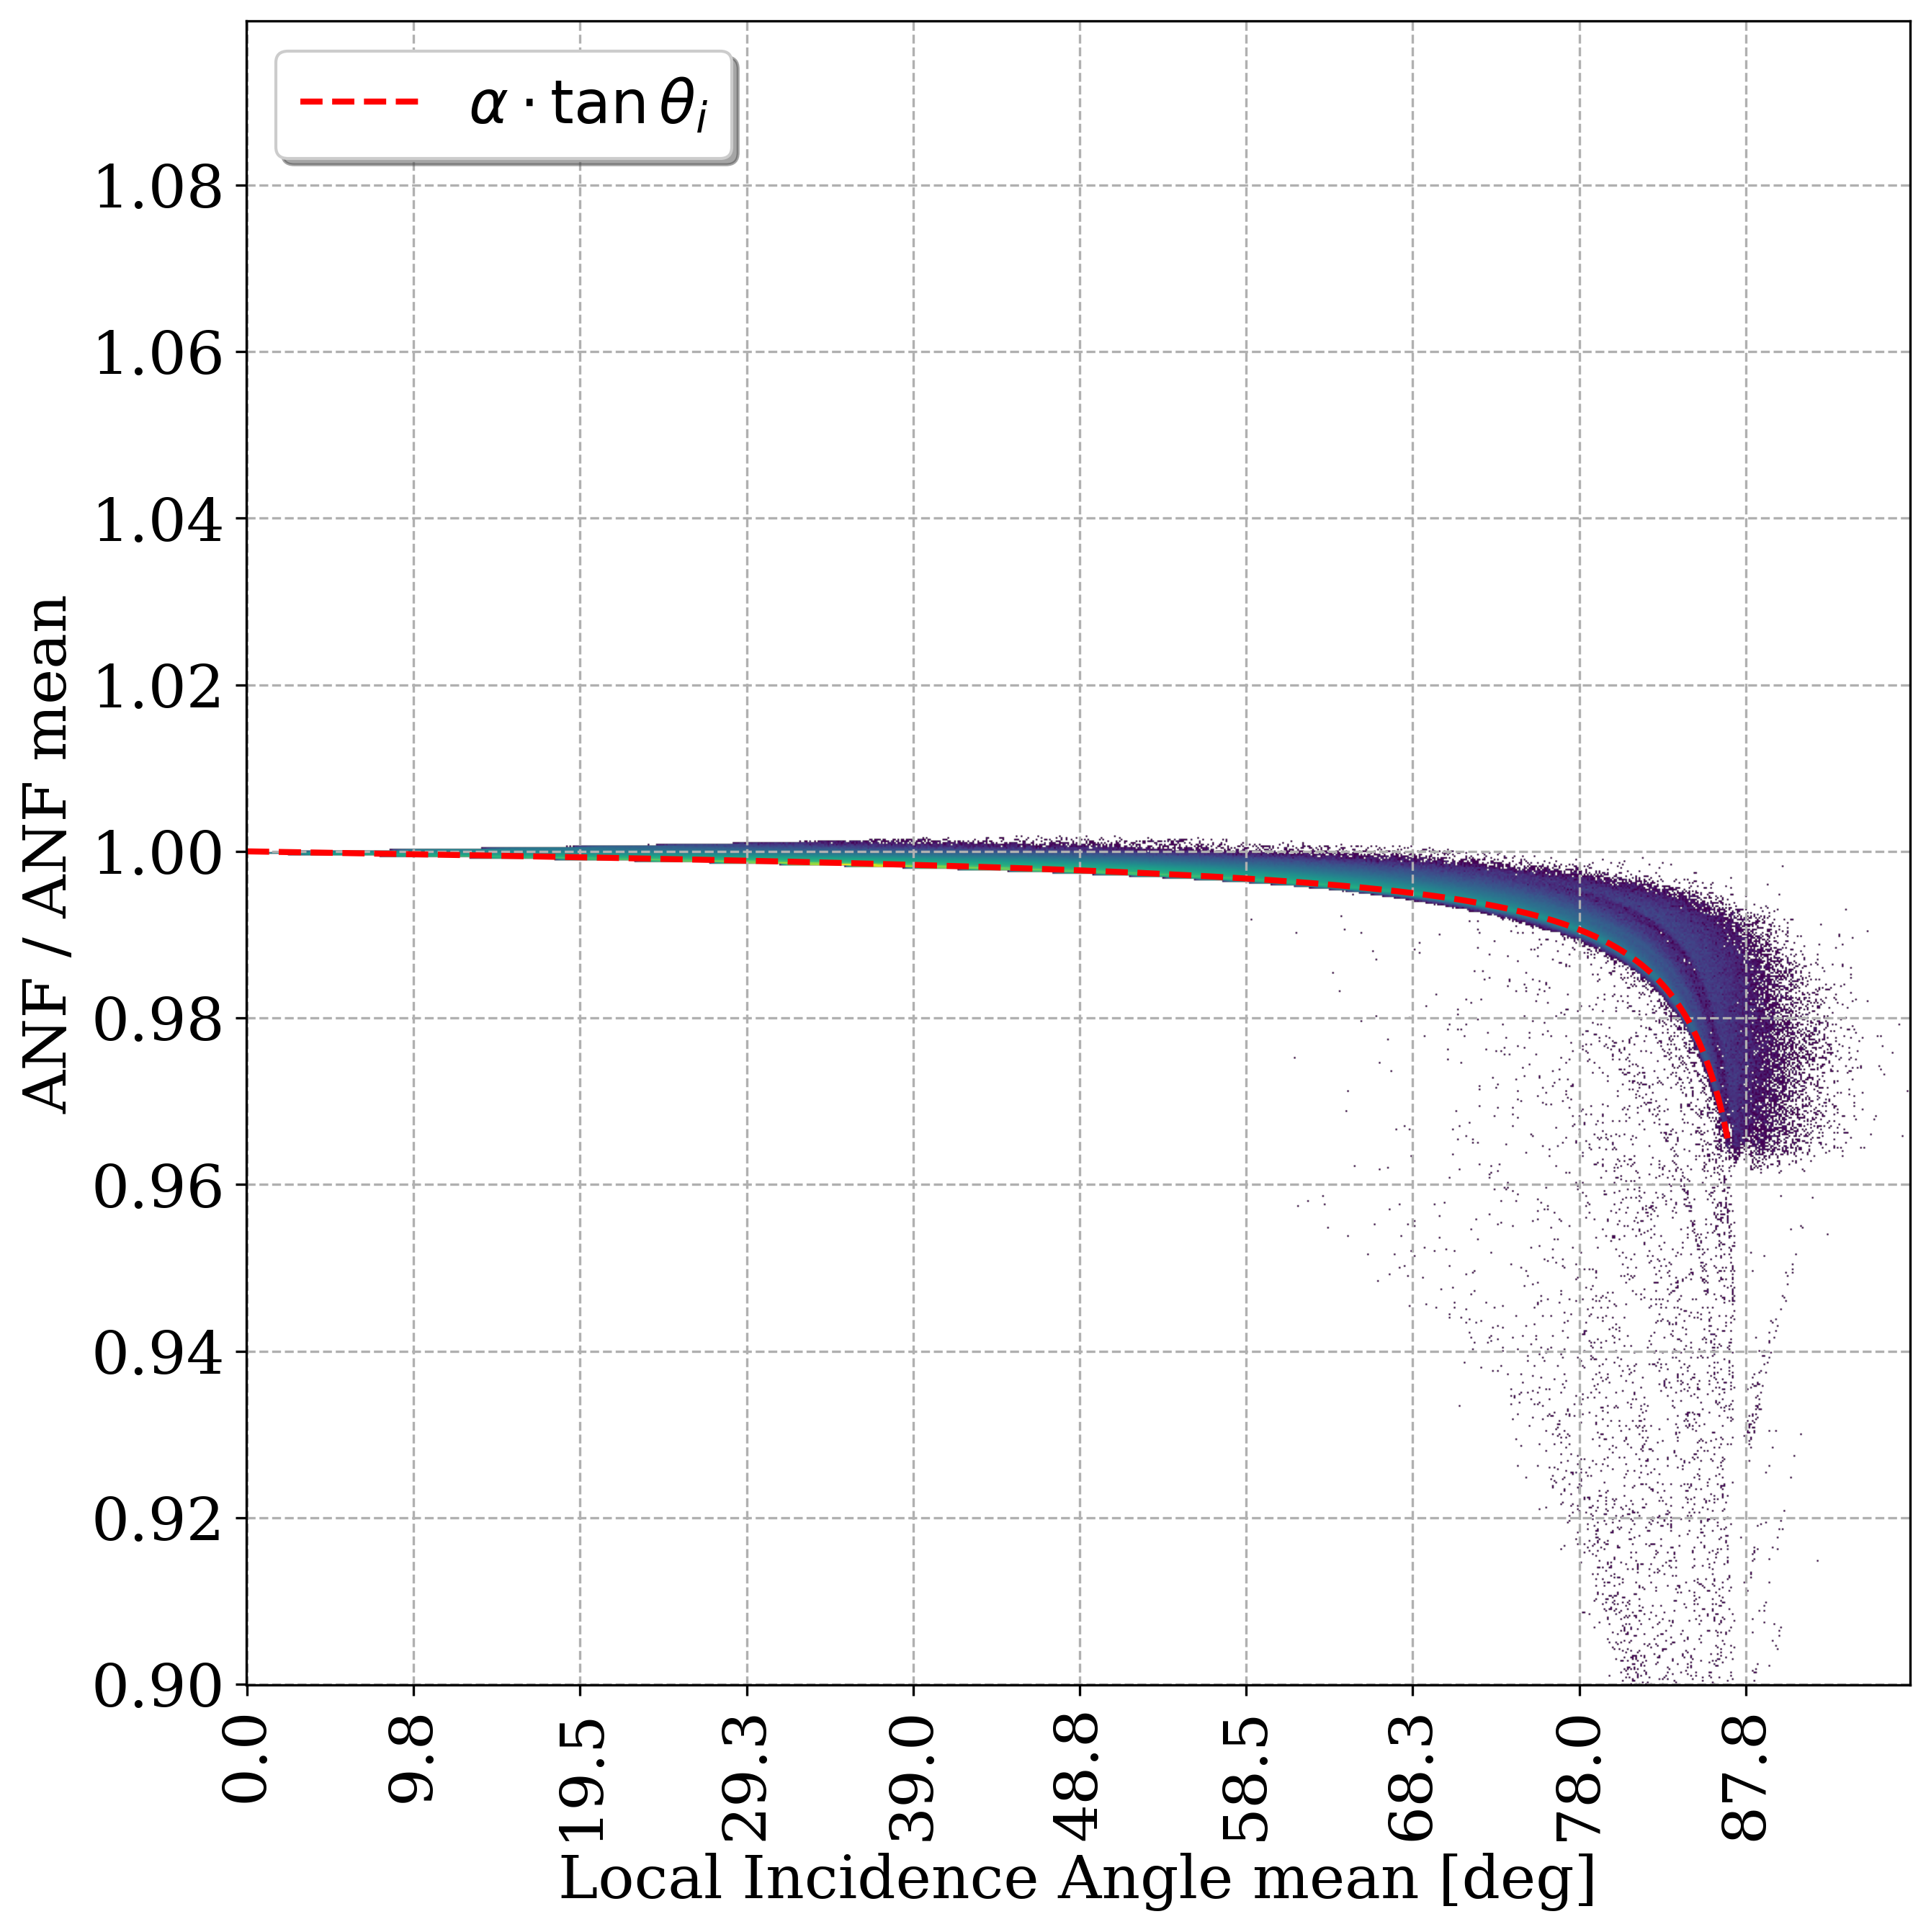
\includegraphics[width=0.9\textwidth]{Figures/nrb/anf_mean_over_lia.png}
  \caption{2D scatter of ANF variability versus local incidence angle. The dashed red line is the first order theoretical approximation from \eqref{eq:ANF_first_ord_B_perp}.}
  \label{fig:ANF_VS_INC_ANGLE}
\end{figure}

\subsection{Computational performance}
\label{sec:nrb_computation}
The generation of NRB products can be based on the processing of each single image independently, with the computation of the specific geometry in correspondence of every new acquisition, or on the processing of stack of images with a co-registration in radar geometry to align all the images with respect to a reference one and the slope flattening andf geocoding with a unique function computed in correspondence of the reference image.

In table \ref{tab:processing_time_single} the absolute time and the percentage of computational cost of the different processing steps with respect to the total amount processing time is reported for a single image. The test refers to an entire Sentinel-1 scene (27 bursts) acquired in IW mode in dual polarization.


\begin{table}[ht]
  \centering
  \caption{Processing time percentage cost vs the total processing time for single image.}
  \label{tab:processing_time_single}
  \begin{tabular}{lll}
    \hline
    Processing step & Processing time [s] & Cost percentage [\%] \\
    \hline
    DEM reprojection    & 63.5 & 9     \\
    Simulation    & 59.4 & 8    \\
    Rasterization  & 413.6 & 56      \\
    Mask shadow    & 108.2 & 15      \\
    Geocoding    & 71.1 & 10      \\
    Mosaic    & 25 & 3      \\
    \hline
  \end{tabular}
\end{table}

The two most time consuming steps are ``Rasterization'' and ``Mask Shadow''. It is worth noting that, by defining a reference geometry, these two steps can be executed only once.

Following this approach and including the image coregistration flow, the processing time percentages is reported in the table \ref{tab:processing_time_single}.

\begin{table}[ht]
  \centering
  \caption{Processing time percentage cost vs the total processing time for co-registration of a stack of 5 images.}
  \label{tab:processing_time_single}
  \begin{tabular}{lll}
    \hline
    Processing step & Processing time [s] & Cost percentage [\%]\\ 
    \hline
    DEM reprojection    & 63.5 & 3     \\
    Simulation   & 430.2 & 20      \\
    Rasterization  & 413.6  & 19      \\
    Mask shadow    & 108.2 & 5      \\
    Coreg   & 695.95 & 33      \\
    Geocoding    & 350 & 16      \\
    Mosaic    & 70.5 & 3      \\
    \hline
  \end{tabular}
\end{table}

Notice that the time to process 5 images is only 2.8 times the one necessary to process a single image with a significant cost reduction. 

\subsection{Criticalities and weakness}
\label{sec:nrb_criticalities}

The generation of NRB products is a well-established process. This type of product is produced routinely using Sentinel-1 data, where a model-based approach is sufficient to correct geometric distortions and compensate for terrain slope.

A critical factor is the alignment between the ANF (simulated backscattering) and the actual SAR image intensity. This alignment depends on the quality of the DEM as well as the accuracy of orbital data and timing. Therefore, it is essential to rely on precise orbital information and timing corrections to account for atmospheric delays (tropospheric and ionospheric).

With Sentinel-1 data, the primary challenge is the timeliness of the availability of these external inputs. For ROSE-L data, additional data-driven corrections are required to compensate for ionospheric effects.

Regarding output resolution, generating products at 10 m is feasible, but speckle becomes the main limiting factor. Based on analyses conducted on Sentinel-1 data, the effective number of looks is approximately 2 in flat areas, and the variability of the backscattering is dominated by speckle. If the final application does not require maximum resolution, lowering the output resolution may be advisable. In addition, this adjustment reduces computational cost proportionally to the increase in the size of the output cell.

The impact of input DEM resolution is primarily confined to areas with steep slopes. Using an area-based approach and comparing input DEM resolutions of 10 m and 30 m—while processing the same image and targeting a 10 m product resolution—the RMSD in steep-slope regions (e.g., the Alps) is less than 1 dB. The RMSD decreases rapidly as the output resolution is lowered.

Orbital tube control is not critical, and two possible mitigation strategies are available:
\begin{itemize} 
    \item \textbf{Independent processing of each image}: the area-based algorithm can be applied individually to each image. In this case, it is crucial to ensure the availability of precise orbital data and SAR image timing information in order to align the ANF with the actual image. 
    \item \textbf{Rescaling the ANF function}: the error in ANF determination can be expressed as a function of the interferometric baseline with respect to the reference geometry and the local incidence angle. By applying a correction specific to each image, it is possible to accurately compensate the ANF without requiring a full computation. 
\end{itemize}


\subsection{Notes on NRB multilook}
\label{sec:nrb_multilook}
Given not normalized weights at $ m $  meters resolution $ v^{m}_{qr} $ for each geographic grid pixel $ q $ and radar pixel $ r $.\\
The not normalized weights at $ n \times m $  meters resolution are given by:
\begin{align}
v^{n \times m}_{pr} = \sum_{q \in p}^{} v^{m}_{qr}
\end{align}
where $q \in p$ denotes all pixels with spacing $m$ that lie within the pixel $p$ with spacing $m \times n$.
The geocoded intensity at $m$ meters resolution is given by:
\begin{align}
g^m_q = \frac{\sum_{r} v^{m}_{qr} c_r}{\sum_{r} v^{m}_{qr}} =\frac{\tilde{g}^m_q}{n_q^m} 
\end{align}
where $c_r$ is the intensity of the radar pixel $r$ and $n_q^m$ is the number of looks of the geogrid pixel $q$.
Then, at $ n \times m $ resolution, the geocoded intensity can be expressed as:
\begin{align}
g^{n \times m}_p &= \frac{\sum_{r} v^{n \times m}_{pr} c_r}{\sum_{r} v^{n \times m}_{pr}} = \frac{\sum_{r}\sum_{q \in p}^{} v^{m}_{qr} c_r}{\sum_{r} \sum_{q \in p}^{} v^{m}_{qr}}=\frac{\sum_{q \in p}^{} \sum_{r}v^{m}_{qr} c_r}{\sum_{q \in p}^{}\sum_{r} v^{m}_{qr}}\\
&= \frac{\sum_{q \in p}^{} \tilde{g}^m_q}{\sum_{q \in p}^{}n_q^m} = \frac{\sum_{q \in p}^{} {g}^m_q \cdot n^m_q}{\sum_{q \in p}^{}n_q^m}
\end{align}

\subsection{Processors configurations}
\label{sec:nrb_proc_config}

\subsubsection{S1-RP}
The following parameters have been used:
\begin{itemize}
    \item chunks to be used during processing: \{"x": 1024, "y": 1024\}
    \item spacing of the resampled DEM: \{"x": 0.3 / 3600, "y": 0.3 / 3600\}
    \item apply\_flattening, whether to apply RTC flattening: True
    \item crs of the resampled DEM: 4326
    \item n\_jobs, number of workers to use: 16
    \item job\_memory, memory allocated for each worker: "16GB"
\end{itemize}
    
\subsubsection{Small C-Code}
Given the zip of a file\\"S1A\_IW\_SLC\_\_1SDV\_20190424T172321\_20190424T172348\_026935\_0307CD\_55E0.SAFE":
\begin{itemize}
    \item unzip the set of input products:  unzip\_list *.zip 
    \item Move each product into “superstructure” to hold the input product with intermediate and output RTC products: mvS1\_list *SAFE
    \item create a backscatter mosaic:
    \begin{itemize}
        \item pushd SLC-IW-20190424\_172321-026935
        \item topsmosBeta SLC-IW-20190424\_172321-026935 1
        \item popd
    \end{itemize}
    \item Run script to create RTC products from a Sentinel-1 IW SLC product:\\ rtcS1slc\_list SLC-IW-20190424\_172321-026935\\
    Line 22 of the rtcS1slc\_list script has been modified in:\\ rtcS1\_dhm\_slc \$f 1 \$UZHRTC\_DIR/DEM/dem 0.3s 1 1000
\end{itemize}
\subsubsection{OPERA-ISCE3}
\begin{itemize}
    \item create a new conda environment: conda create -n RTC -c conda-forge python=3.11.12
    \item activate your conda environment: conda activate RTC
    \item download the source code:\\ git clone -b v1.0.2 https://github.com/opera-adt/RTC.git
    \item install isce3: conda install -c conda-forge isce3==0.15.0
    \item download s1-reader:\\
    git clone -b v0.2.4 https://github.com/isce-framework/s1-reader.git
    \item install s1-reader:\\conda env update -n RTC -f s1-reader/environment.yaml\\
    python -m pip install ./s1-reader
    \item install RTC:
    python -m pip install ./RTC
    \item launch the software: rtc\_s1.py rtc\_s1\_.yaml
\end{itemize}
An example of the configuration file used is provided below:
\lstinputlisting[language=yaml]{Figures/nrb/rtc_s1.yaml}